%  path0 <- "c:/data/GUK/"; path <- paste0(path0, "analysis/"); setwd(pathprogram <- paste0(path, "program/")); system("recycle c:/data/GUK/analysis/program/cache/PermutationTests5/"); library(knitr); knit("PermutationTests5.rnw", "PermutationTests5.tex"); system("platex PermutationTests5"); system("dvipdfmx PermutationTests5")

\input{c:/seiro/settings/Rsetting/knitrPreamble/knitr_preamble.rnw}
\renewcommand\Routcolor{\color{gray30}}
\newtheorem{finding}{Finding}[section]
\makeatletter
\g@addto@macro{\UrlBreaks}{\UrlOrds}
\newcommand\gobblepars{%
    \@ifnextchar\par%
        {\expandafter\gobblepars\@gobble}%
        {}}
\newenvironment{lightgrayleftbar}{%
  \def\FrameCommand{\textcolor{lightgray}{\vrule width 1zw} \hspace{10pt}}% 
  \MakeFramed {\advance\hsize-\width \FrameRestore}}%
{\endMakeFramed}
\newenvironment{palepinkleftbar}{%
  \def\FrameCommand{\textcolor{palepink}{\vrule width 1zw} \hspace{10pt}}% 
  \MakeFramed {\advance\hsize-\width \FrameRestore}}%
{\endMakeFramed}
\makeatother
\usepackage{caption}
\usepackage{setspace}
\usepackage{framed}
\captionsetup[figure]{font={stretch=.6}} 
\def\pgfsysdriver{pgfsys-dvipdfm.def}
\usepackage{tikz}
\usetikzlibrary{calc, arrows, decorations, decorations.pathreplacing, backgrounds}
\usepackage{adjustbox}
\tikzstyle{toprow} =
[
top color = gray!20, bottom color = gray!50, thick
]
\tikzstyle{maintable} =
[
top color = blue!1, bottom color = blue!20, draw = white
%top color = green!1, bottom color = green!20, draw = white
]
\tikzset{
%Define standard arrow tip
>=stealth',
%Define style for different line styles
help lines/.style={dashed, thick},
axis/.style={<->},
important line/.style={thick},
connection/.style={thick, dotted},
}


\begin{document}
\setlength{\baselineskip}{12pt}








\hfil Permutation tests\\

\hfil\MonthDY\\
\hfil{\footnotesize\currenttime}\\

\hfil Seiro Ito

\setcounter{tocdepth}{3}
\tableofcontents

\setlength{\parindent}{1em}
\vspace{2ex}


% This is a child file of PermutationTests5.rnw
Use the `trimmed' sample (has all 800 members) rather than the `initial' sample (has only 776 members after dropping members who received loans only twice). To set to the trimmed sample, set the parameter \textsf{UseTrimmedSample} to T.
\begin{Schunk}
\begin{Sinput}
UseTrimmedSample <- T
TestMedian <- F
\end{Sinput}
\end{Schunk}

The majority of descriptive statistics are related to assets. We base our descriptive statistics on the asset data.

\begin{Schunk}
\begin{Sinput}
source(paste0(pathprogram, "ComputeNetAssetsANCOVA.R"))
\end{Sinput}
\begin{Soutput}


Number of obs by Arm and attrition
             AttritIn
Arm             2   3   4   9 Sum
  traditional   6   4  20 144 174
  large         5   2   1 192 200
  large grace  22   3   3 171 199
  cattle        5   5  13 177 200
  Sum          38  14  37 684 773


Number of obs by membership status and attrition
                      AttritIn
BStatus                  2   3   4   9 Sum
  borrower               8   6   8 578 600
  pure saver             0   0   0   0   0
  individual rejection   9   4   1  75  89
  group rejection        9   4   0  55  68
  rejection by flood    12   0  28   0  40
  Sum                   38  14  37 708 797
\end{Soutput}
\end{Schunk}
\begin{Schunk}
\begin{Sinput}
#  trimmed sample are data before dropping 26 traditional HHs.
ar <- readRDS(paste0(pathsaveHere, DataFileNames[3], "Trimmed.rds"))
arA <- readRDS(paste0(pathsaveHere, DataFileNames[2], "Trimmed.rds"))
ass <- readRDS(paste0(pathsaveHere, DataFileNames[4], "Trimmed.rds"))
lvo <- readRDS(paste0(pathsaveHere, DataFileNames[5], "Trimmed.rds"))
NeA1R <- readRDS(paste0(pathsaveHere, "NetAssetsANCOVATrimmed.rds"))
# NeA1R2 drops (from NeA1R) 24 members in trad who were disbursed loans only twice or once
NeA1R2 <- readRDS(paste0(pathsaveHere, "NetAssetsANCOVA.rds"))
rsk <- readRDS(paste0(pathsaveHere, "RiskPreferences.rds"))
rsk2 <- rsk[, .(hhid, RiskPrefVal, TimePref1Val, TimePref2Val, PresentBias)]
if (Only800) ar <- ar[o800 == 1L, ]
addmargins(table(ar[tee == 1, .(Arm)]))
\end{Sinput}
\begin{Soutput}
Arm
traditional       large large grace      cattle         Sum 
        200         200         200         200         800 
\end{Soutput}
\end{Schunk}
There are 24 members with TradGroup = twice, double. They were dropped from estimation sample. If \textsf{UseTrimmedSample==T}, attrition is based on all 800 members, if \textsf{F}, attrition is analysed using 776 members. We use the `initial' sample (has only 776 members after dropping members who received loans only twice), not the `trimmed' sample (has all 800 members). \gobblepars
\begin{Schunk}
\begin{Sinput}
#To set to the trimmed sample, set the parameter \textsf{UseTrimmedSample} to T. Here, we set to F.
#Trimmed sample: Has all 800 HHs. Initial sample: Has 776 HHs.
UseTrimmedSample <- F
TestMedian <- F
\end{Sinput}
\end{Schunk}
\begin{Schunk}
\begin{Sinput}
cat("UseTrimmedSample is", UseTrimmedSample, "\n")
\end{Sinput}
\begin{Soutput}
UseTrimmedSample is FALSE 
\end{Soutput}
\begin{Sinput}
if (!UseTrimmedSample) 
  ar <- ar[!grepl("tw|dou", TradGroup), ]
addmargins(table0(ar[o800 == 1L & tee == 1, .(Tee, AttritIn)]))
\end{Sinput}
\begin{Soutput}
     AttritIn
Tee     2   3   4   9 Sum
  1    41   0   0   0  41
  2     0  14   0   0  14
  3     0   0  37   0  37
  4     0   0   0 684 684
  Sum  41  14  37 684 776
\end{Soutput}
\end{Schunk}
Out of 776 members, there are 92 members who attrited.
\begin{Schunk}
\begin{Sinput}
addmargins(table0(ar[tee==1 & o800==1 & AttritIn<9, .(BStatus,AttritIn)]))
\end{Sinput}
\begin{Soutput}
                      AttritIn
BStatus                 2  3  4 Sum
  borrower              8  6  8  22
  pure saver            0  0  0   0
  individual rejection 10  4  1  15
  group rejection      11  4  0  15
  rejection by flood   12  0 28  40
  Sum                  41 14 37  92
\end{Soutput}
\begin{Sinput}
#addmargins(table(ar[mid == 1 & Time == 1, .(BStatus, Arm)]), 1:2, sum, T)
#addmargins(table(ar[mid == 1 & Time == 4, .(BStatus, Arm)]), 1:2, sum, T)
# "ar" is roster
# AttritIn is created as below in read_cleaned_data.rnw
# (465): xid[, AttritIn := 9L]
# (466): xid[grepl("^En|^2nd and 4", missing_followup), AttritIn := 4L]
# (467): xid[grepl("^3rd and 4", missing_followup), AttritIn := 3L]
# (468): xid[grepl("^2.*3.*4", missing_followup), AttritIn := 2L]
\end{Sinput}
\end{Schunk}
\begin{Schunk}
\begin{Sinput}
ar[, Tee := max(survey), by = hhid]
arA[, Tee := max(survey), by = hhid]
ass[, Tee := max(survey), by = hhid]
lvo[, Tee := max(survey), by = hhid]
\end{Sinput}
\end{Schunk}
%Correct \textsf{AttritIn} for these nrow(ar[grepl("tw|dou", TradGroup) & tee == 1, ]) members. Keep only the 1st obs for all members.
\begin{Schunk}
\begin{Sinput}
#addmargins(table(ar[tee == 1 & grepl("tw|dou", TradGroup), AttritIn]))
#ar[Tee == 1 & AttritIn == 9 & grepl("tw|dou", TradGroup), AttritIn := 2L]
\end{Sinput}
\end{Schunk}
\begin{Schunk}
\begin{Sinput}
psas <- ass[o800 == 1 & tee == 1, 
  .(hhid, tee, NLHAssetAmount, PAssetAmount)]
pslv <- lvo[o800 == 1 & tee == 1, 
  .(hhid, tee, TotalImputedValue, NumCows)]
nne <- NeA1R[o800 == 1 & tee == 1, 
  # NetBroadValue is similar to NetValue, so drop it.
  .(hhid, tee, NetValue , #NarrowNetValue, 
  NetBroadValue
  #, RNetValue, RNarrowNetValue, RNetBroadValue
  )]
\end{Sinput}
\end{Schunk}
\begin{Schunk}
\begin{Sinput}
source(paste0(pathprogram, "AttritionPermutationTableHeaders5.R"))
armerge <- ar[, c("groupid", "hhid", "mid", "o800", "TradGroup", 
  "BStatus", "AttritIn", "survey", "tee", "Time", vartobetested[1:5]), with = F]
armerge[, En := 1:.N, by = .(hhid, Time)]
armerge[, Tee := .N, by = .(hhid, mid, Time)]
armerge <- armerge[En == 1 & Time == 1 & o800 == 1, ]
as <- merge(armerge, psas, by = c("hhid", "tee"), all.x = T)
asl <- merge(as, pslv, by = c("hhid", "tee"), all.x = T)
asln <- merge(asl, nne, by = c("hhid", "tee"), all.x = T)
asv <- merge(asln, rsk2, by = "hhid", all.x = T)
addmargins(table0(asv[!grepl("tw|dou", TradGroup), .(Arm, AttritIn)]))
\end{Sinput}
\begin{Soutput}
             AttritIn
Arm             2   3   4   9 Sum
  traditional   8   4  20 144 176
  large         5   2   1 192 200
  large grace  23   3   3 171 200
  cattle        5   5  13 177 200
  Sum          41  14  37 684 776
\end{Soutput}
\begin{Sinput}
# keep only rational respondents of risk preferences
\end{Sinput}
\end{Schunk}
\begin{Schunk}
\begin{Sinput}
# use tee==4 to define attrition, where tee is survey round in asset and livestock 
# while tee in roster is meeting number (must rename survey to tee)
asv[, Attrited := 0L]
asv[hhid %in% hhid[AttritIn < 9], Attrited := 1L]
addmargins(table0(asv[!grepl("tw|dou", TradGroup), .(Arm, Attrited)]))
\end{Sinput}
\begin{Soutput}
             Attrited
Arm             0   1 Sum
  traditional 144  32 176
  large       192   8 200
  large grace 171  29 200
  cattle      177  23 200
  Sum         684  92 776
\end{Soutput}
\begin{Sinput}
asv[, c("Rejected", "GRejected", "IRejected") := 0L]
asv[grepl("^i.*rej", BStatus), IRejected := 1L]
asv[grepl("^g.*rej", BStatus), GRejected := 1L]
asv[IRejected == 1L | GRejected == 1L, Rejected := 1L]
asv[, Active := 1L]
asv[Attrited == 1 | Rejected == 1, Active := 0L]
asv[, CompletePanel := F]
asv[hhid %in% intersect(hhid[tee == 1 & !is.na(NetValue)], hhid[tee == 4 & !is.na(NetValue)]),
  CompletePanel := T]
saveRDS(asv, paste0(pathsaveHere, "DestatData.rds"))
\end{Sinput}
\end{Schunk}
Attrition of members who were not affected by floods.
\begin{Schunk}
\begin{Sinput}
asv <- readRDS(paste0(pathsaveHere, "DestatData.rds"))
addmargins(table0(asv[!grepl("flo", BStatus) & Rejected == 0, .(Attrited, Arm)]))
\end{Sinput}
\begin{Soutput}
        Arm
Attrited traditional large large grace cattle Sum
     0            83   164         160    147 554
     1             2     7           7      6  22
     Sum          85   171         167    153 576
\end{Soutput}
\begin{Sinput}
# these are HHs with two disbursements under traditional; read_admin_data.rnw(472)
# adw[(loanamount1st == 5600 & loanamount2nd == 5600 & loanamount3rd == 5600) |
#   (!is.na(DisDate1) & !is.na(DisDate2) & !is.na(DisDate3)), 
#   TradGroup := "planned"]
# adw[loanamount1st == 5600 & loanamount2nd == 11200, 
#   TradGroup := "double"]
# adw[(loanamount1st == 7840 & loanamount2nd == 8960) | 
#   (!is.na(DisDate1) & !is.na(DisDate2) & is.na(DisDate3)), 
#   TradGroup := "twice"]
# adw[, TradGroup := factor(TradGroup, levels = c("planned", "twice", "double"))]
\end{Sinput}
\end{Schunk}
\begin{Schunk}
\begin{Sinput}
# data to use in each tests: TradNonTradAttrited, AttritedInTrad, TradNonTradRejected, IRejected, RejectedInTrad, RejectedInNonTrad
# drop 2 loan receivers
asv1 <- asv[!grepl("tw|dou", TradGroup), ]
# drop group rejecters
asv2 <- asv[!grepl("gr", BStatus), ]
# drop 2 loan receivers and group rejecters
asv3 <- asv[!grepl("gr", BStatus) & !grepl("tw|dou", TradGroup), ]
asvT <- asv[grepl("tra", Arm), ]
asvNT <- asv[!grepl("tra", Arm), ]
# data to be used for each tested variable
# vartobetested is defined in AttritionPermutationTableHeaders5.R in FormSample.rnw
datalist <- rep("asv", length(vartobetested))
datalist1 <- paste0(datalist, 1) # drop 2 loan receivers
datalist2 <- paste0(datalist, 2) # drop group rejecters
datalist3 <- paste0(datalist, 3) # drop 2 loan receivers and group rejecters
datasets <- "asv"
datasets1 <- paste0(datasets, 1)
datasets2 <- paste0(datasets, 2)
datasets3 <- paste0(datasets, 3)
for (k in 1:3) {
  addchar <- c("f", "t", "j")[k]
  Datasets <- get(paste0("datasets", c("", 1, 2)[k]))
  for (dd in Datasets) {
    xdd <- get(dd)
    # all members all arms: attrited vs. nonattrited
    xa <- xdd
    assign(paste0(dd, "a", addchar), xa)
    # all in trad: attrition vs. nonattrition
    xTa <- xdd[grepl("trad", Arm), ]
    assign(paste0(dd, "Ta", addchar), xTa)
    # all in nontrad: attrition vs. nonattrition
    xNTa <- xdd[!grepl("trad", Arm), ]
    assign(paste0(dd, "NTa", addchar), xNTa)
    # attrited members in all arms: trad vs. nontrad
    xTNTa <- xdd[Attrited == 1L, ]
    xTNTa[, TradArm := 1L]; xTNTa[!grepl("trad", Arm), TradArm := 0L]
    assign(paste0(dd, "TNTa", addchar), xTNTa)
    # all members except flood victims: attrited vs. nonattrited
    xNFa <- xdd[!grepl("floo", BStatus), ]
    assign(paste0(dd, "NFa", addchar), xNFa)
    # all except flood victims in trad: attrition vs. nonattrition
    xNFTa <- xdd[!grepl("floo", BStatus) & grepl("trad", Arm), ]
    assign(paste0(dd, "NFTa", addchar), xNFTa)
    # all except flood victims in nontrad: attrition vs. nonattrition
    xNFNTa <- xdd[!grepl("floo", BStatus) & !grepl("trad", Arm), ]
    assign(paste0(dd, "NFNTa", addchar), xNFNTa)
    # attrited members except flood victims in all arms: trad vs. nontrad
    xNFTNTa <- xdd[!grepl("floo", BStatus) & Attrited == 1L, ]
    xNFTNTa[, TradArm := 1L]; xNFTNTa[!grepl("trad", Arm), TradArm := 0L]
    assign(paste0(dd, "NFTNTa", addchar), xNFTNTa)
    # attrited members except flood victims in all arms: cow vs. noncow
    xNFCNCa <- xdd[!grepl("floo", BStatus) & Attrited == 1L, ]
    xNFCNCa[, CowArm := 1L]; xNFCNCa[!grepl("cow", Arm), CowArm := 0L]
    assign(paste0(dd, "NFCNCa", addchar), xNFCNCa)
    # attrited members except flood victims: cow vs. large grace
    xNFCGa <- xdd[!grepl("floo", BStatus) & grepl("cow|gr", Arm) & Attrited == 1L, ]
    xNFCGa[, CowArm := 1L]; xNFCGa[!grepl("cow", Arm), CowArm := 0L]
    assign(paste0(dd, "NFCGa", addchar), xNFCGa)
    # active/surviving (neither attrited nor rejected) members except flood victims 
    # (these people are considered not fit for the offered program)
    # active/survival in all arms
    xs <- xdd
    assign(paste0(dd, "s", addchar), xs)
    # active in trad: attrition vs. nonattrition
    xTs <- xdd[grepl("trad", Arm), ]
    assign(paste0(dd, "Ts", addchar), xTs)
    # active in nontrad: attrition vs. nonattrition
    xNTs <- xdd[!grepl("trad", Arm), ]
    assign(paste0(dd, "NTs", addchar), xNTs)
    # active members in all arms: trad vs. nontrad
    xTNTs <- xdd[Active == 1L, ]
    xTNTs[, TradArm := 1L]; xTNTs[!grepl("trad", Arm), TradArm := 0L]
    assign(paste0(dd, "TNTs", addchar), xTNTs)
    # active members: cow vs. noncow
    xCNCs <- xdd[!grepl("floo", BStatus) & Active == 1L, ]
    xCNCs[, CowArm := 1L]; xCNCs[!grepl("cattle", Arm), CowArm := 0L]
    assign(paste0(dd, "CNCs", addchar), xCNCs)
    # active members: cow vs. lsge grace
    xCGs <- xdd[!grepl("floo", BStatus) & grepl("cattle|gr", Arm) & Active == 1L, ]
    xCGs[, CowArm := 1L]; xCGs[!grepl("cattle", Arm), CowArm := 0L]
    assign(paste0(dd, "CGs", addchar), xCGs)
    # all rejection all arms: rejected vs. nonrejected
    xr <- xdd
    assign(paste0(dd, "r", addchar), xr)
    # all rejection in trad: rejected vs. nonrejected
    xTr <- xdd[grepl("trad", Arm), ]
    assign(paste0(dd, "Tr", addchar), xTr)
    # all rejection in nontrad: rejected vs. nonrejected
    xNTr <- xdd[!grepl("trad", Arm), ]
    assign(paste0(dd, "NTr", addchar), xNTr)
    # all rejection: trad rejecetd vs. nontrad rejected
    xTNTr <- xdd[Rejected == 1L, ]
    xTNTr[, TradArm := 1L]; xTNTr[!grepl("trad", Arm), TradArm := 0L]
    assign(paste0(dd, "TNTr", addchar), xTNTr)
    # all rejection: cattle rejecetd vs. noncattle rejected
    xCNCr <- xdd[Rejected == 1L, ]
    xCNCr[, CowArm := 1L]; xCNCr[!grepl("cattle", Arm), CowArm := 0L]
    assign(paste0(dd, "CNCr", addchar), xCNCr)
    # all rejection: cattle rejecetd vs. large grace rejected
    xCLGr <- xdd[grepl("cattle|gr", Arm) & Rejected == 1L, ]
    xCLGr[, CowArm := 1L]; xCLGr[!grepl("cattle", Arm), CowArm := 0L]
    assign(paste0(dd, "CLGr", addchar), xCLGr)
    # all acceptance: cattle accepted vs. noncattle accepted
    xCNCa <- xdd[Rejected == 0L, ]
    xCNCa[, CowArm := 1L]; xCNCa[!grepl("cattle", Arm), CowArm := 0L]
    assign(paste0(dd, "CNCa", addchar), xCNCa)
    # all acceptance: cattle accepted vs. large grace accepted
    xCLGa <- xdd[grepl("cattle|gr", Arm) & Rejected == 0L, ]
    xCLGa[, CowArm := 1L]; xCLGa[!grepl("cattle", Arm), CowArm := 0L]
    assign(paste0(dd, "CLGa", addchar), xCLGa)
    # group rejection in all arms: rejected vs. nonrejected
    xgr <- xdd
    assign(paste0(dd, "gr", addchar), xgr)
    # group rejection in trad: rejecters vs. nonrejecters
    xTgr <- xdd[grepl("tra", Arm), ]
    assign(paste0(dd, "Tgr", addchar), xTgr)
    # group rejection in nontrad: rejecters vs. nonrejecters
    xNTgr <- xdd[!grepl("tra", Arm), ]
    assign(paste0(dd, "NTgr", addchar), xNTgr)
    # group rejection: trad rejecters vs. nontrad rejecters
    xTNTgr <- xdd[GRejected == 1L, ]
    xTNTgr[, TradArm := 1L]; xTNTgr[!grepl("trad", Arm), TradArm := 0L]
    assign(paste0(dd, "TNTgr", addchar), xTNTgr)
    # individual rejection in all arms: rejected vs. nonrejected
    # individual rejecters vs. all except group rejecters
    # group rejecters are excluded because they preceded indiv rejection
    xir <- xdd[!grepl("gr", BStatus), ]
    assign(paste0(dd, "ir", addchar), xir)
    # individual rejection in trad: rejecters vs. nonrejecters
    xTir <- xdd[grepl("tra", Arm) & !grepl("gr", BStatus), ]
    assign(paste0(dd, "Tir", addchar), xTir)
    # individual rejection in nontrad: rejecters vs. nonrejecters
    xNTir <- xdd[!grepl("tra", Arm) & !grepl("gr", BStatus), ]
    assign(paste0(dd, "NTir", addchar), xNTir)
    # individual rejection: trad rejecters vs. nontrad rejecters
    xTNTir <- xdd[!grepl("gr", BStatus) & Rejected == 1L, ]
    xTNTir[, TradArm := 1L]; xTNTir[!grepl("trad", Arm), TradArm := 0L]
    assign(paste0(dd, "TNTir", addchar), xTNTir)
    # trad group rejecters vs. nontrad participants
    xTNTgrp <- xdd[(grepl("gr", BStatus) & grepl("trad", Arm) & Rejected == 1L) |
      (grepl("bo", BStatus) & !grepl("trad", Arm)), ]
    xTNTgrp[, TradArm := 1L]; xTNTgrp[!grepl("trad", Arm), TradArm := 0L]
    assign(paste0(dd, "TNTgrp", addchar), xTNTgrp)
    # trad group vs. nontrad group
    xTNTrandom <- xdd
    xTNTrandom[, TradArm := 1L]; xTNTrandom[!grepl("trad", Arm), TradArm := 0L]
    assign(paste0(dd, "TNTrandom", addchar), xTNTrandom)
  }
}
\end{Sinput}
\end{Schunk}
\begin{Schunk}
\begin{Sinput}
# data names: ..af, ..rf  (full), ..at, ..rt (drop 2 loan receivers), ..aj, ..rj (drop group rejeceters)
# data to use: datalist (full), datalist1 (drop 2 loan receivers), datalist2 (drop group rejeceters)
library(coin)
PM <- vector(mode = "list", length = 3)
for (k in 1:3) {
  addchar <- c("f", "t", "j")[k]
  dataList <- eval(parse(text=paste0("datalist", c("", 1:2))[k]))
  if (addchar == "j") M <- 9 else M <- length(selection.criteria)
  Pm <- vector(mode = "list", length = M)
  for (m in 1:M) {
    set.seed(100+m)
    if (grepl("^Attrited$", addtofilename[m])) 
      DataList <- gsub("$", paste0("a", addchar), dataList) else 
    if (grepl("^AttritedInTrad", addtofilename[m])) 
      DataList <- gsub("$", paste0("Ta", addchar), dataList) else 
    if (grepl("^AttritedInNonTrad", addtofilename[m])) 
      DataList <- gsub("$", paste0("NTa", addchar), dataList) else 
    if (grepl("^TradNonTradAttrited$", addtofilename[m])) 
      DataList <- gsub("$", paste0("TNTa", addchar), dataList) else 
    if (grepl("^NonFloodAttrited$", addtofilename[m])) 
      DataList <- gsub("$", paste0("NFa", addchar), dataList) else 
    if (grepl("^NonFloodAttritedInTrad$", addtofilename[m])) 
      DataList <- gsub("$", paste0("NFTa", addchar), dataList) else 
    if (grepl("^NonFloodAttritedInNonTrad$", addtofilename[m])) 
      DataList <- gsub("$", paste0("NFNTa", addchar), dataList) else 
    if (grepl("^NonFloodTradNonTradAttrited$", addtofilename[m])) 
      DataList <- gsub("$", paste0("NFTNTa", addchar), dataList) else 
    if (grepl("^NonFloodAttritedCowN", addtofilename[m])) 
      DataList <- gsub("$", paste0("NFCNCa", addchar), dataList) else 
    if (grepl("^NonFloodAttritedCowL", addtofilename[m])) 
      DataList <- gsub("$", paste0("NFCGa", addchar), dataList) else 
    if (grepl("^Active$", addtofilename[m])) 
      DataList <- gsub("$", paste0("s", addchar), dataList) else 
    if (grepl("^ActiveInTrad", addtofilename[m])) 
      DataList <- gsub("$", paste0("Ts", addchar), dataList) else 
    if (grepl("^ActiveInNonTrad", addtofilename[m])) 
      DataList <- gsub("$", paste0("NTs", addchar), dataList) else 
    if (grepl("^ActiveTradNonTrad", addtofilename[m])) 
      DataList <- gsub("$", paste0("TNTs", addchar), dataList) else 
    if (grepl("^ActiveCowN", addtofilename[m]))
      DataList <- gsub("$", paste0("CNCs", addchar), dataList) else 
    if (grepl("^ActiveCowL", addtofilename[m])) 
      DataList <- gsub("$", paste0("CGs", addchar), dataList) else 
    if (grepl("^Random", addtofilename[m])) 
      DataList <- gsub("$", paste0("TNTrandom", addchar), dataList) else 
    if (grepl("^Rejected$", addtofilename[m])) 
      DataList <- gsub("$", paste0("r", addchar), dataList) else 
    if (grepl("^Rej.*InTrad$", addtofilename[m])) 
      DataList <- gsub("$", paste0("Tr", addchar), dataList) else 
    if (grepl("^Rej.*InNonTrad$", addtofilename[m])) 
      DataList <- gsub("$", paste0("NTr", addchar), dataList) else 
    if (grepl("^TradNonTradR", addtofilename[m])) 
      DataList <- gsub("$", paste0("TNTr", addchar), dataList) else 
    if (grepl("^GRejected$", addtofilename[m])) 
      DataList <- gsub("$", paste0("gr", addchar), dataList) else 
    if (grepl("^GRej.*InTrad$", addtofilename[m])) 
      DataList <- gsub("$", paste0("Tgr", addchar), dataList) else 
    if (grepl("^GRej.*InNonTrad$", addtofilename[m])) 
      DataList <- gsub("$", paste0("NTgr", addchar), dataList) else 
    if (grepl("^TradNonTradGR", addtofilename[m])) 
      DataList <- gsub("$", paste0("TNTgr", addchar), dataList) else 
    if (grepl("^IRejected$", addtofilename[m])) 
      DataList <- gsub("$", paste0("ir", addchar), dataList) else 
    if (grepl("^IRej.*InTrad$", addtofilename[m])) 
      DataList <- gsub("$", paste0("Tir", addchar), dataList) else 
    if (grepl("^IRej.*InNonTrad$", addtofilename[m])) 
      DataList <- gsub("$", paste0("NTir", addchar), dataList) else 
    if (grepl("^TradNonTradIR", addtofilename[m])) 
      DataList <- gsub("$", paste0("TNTir", addchar), dataList) else 
    if (grepl("^GRejectedTradPar", addtofilename[m])) 
      DataList <- gsub("$", paste0("TNTgrp", addchar), dataList) else 
    if (grepl("^RejectedCowN", addtofilename[m])) 
      DataList <- gsub("$", paste0("CNCr", addchar), dataList) else 
    if (grepl("^RejectedCowLa", addtofilename[m])) 
      DataList <- gsub("$", paste0("CLGr", addchar), dataList) else 
    if (grepl("^AcceptedCowN", addtofilename[m])) 
      DataList <- gsub("$", paste0("CNCa", addchar), dataList) else 
    if (grepl("^AcceptedCowLa", addtofilename[m])) 
      DataList <- gsub("$", paste0("CLGa", addchar), dataList) else 
      DataList <- gsub("$", addchar, dataList)
    pmresults <- permmedian <- vector(mode = "list", length(vartobetested))
    for (i in 1:length(vartobetested)) {
      # if specific arm is selected, Arm is not compared in permutation
      if (grepl("Trad$|TradArm|Cow", addtofilename[m]) & 
        vartobetested[i] == "Arm") next
      pmdata <- get(DataList[i])
      # drop NAs in vartobetested[i]
      pmdata <- pmdata[!is.na(eval(parse(text=vartobetested[i]))), ]
      # NULL if vartobetested[i] has uniform values or 
      # selection.criteria[m] has has uniform values (otherwise returns an error)
      if (length(unique(unlist(pmdata[, vartobetested[i], with = F]))) == 1|
          length(unique(unlist(pmdata[, selection.criteria[m], with = F]))) == 1) 
        pmresults[[i]] <- NULL else 
        pmresults[[i]] <- independence_test(eval(parse(text=
          paste(vartobetested[i], "~ as.factor(", selection.criteria[m], ")")
          )), 
          data = pmdata, 
          distribution = approximate(nresample=PermRepTimes))
      if (!TestMedian) next
      if (vartobetested[i] == "Arm" | 
        length(unique(unlist(pmdata[, vartobetested[i], with = F]))) == 1 |
        length(unique(unlist(pmdata[, selection.criteria[m], with = F]))) == 1) 
        permmedian[[i]] <- NULL else 
        permmedian[[i]] <- median_test(eval(parse(text=
          paste(vartobetested[i], "~ as.factor(", selection.criteria[m], ")"))), 
          data = pmdata,
          mid.score = "0.5",
          distribution = approximate(nresample=PermRepTimes))
    }
    #pmresults[[1]]@statistic@teststatistic
    Pmtresults <- NULL
    for (i in 1:length(vartobetested)) 
    {
      if (grepl("Trad$|TradArm|Cow", addtofilename[m]) & 
        vartobetested[i] == "Arm") next
      z <- get(DataList[i])
      z <- z[!is.na(eval(parse(text=vartobetested[i]))), ]
      if (vartobetested[i] == "Arm") {
        Pmtresults <- rbind(Pmtresults, 
          c(vartobetested[i], 
            sum(!grepl("trad", unlist(z[eval(parse(text = selection.criteria[m])) == 0L, 
              vartobetested[i], with = F])))/
              nrow(z[eval(parse(text = selection.criteria[m])) == 0L, ]),
            sum(!grepl("trad", unlist(z[eval(parse(text = selection.criteria[m])) == 1L, 
              vartobetested[i], with = F])))/
              nrow(z[eval(parse(text = selection.criteria[m])) == 1L, ]),
            midpvalue(pmresults[[i]]), 
            pvalue_interval(pmresults[[i]])))
      } else if (length(unique(unlist(z[, vartobetested[i], with = F]))) == 1) 
      {
        # if both groups have no different values, 
        # use 0 for all zero entries or 1 for unique nonzero entries
        if (allzerovalues <- unique(unlist(z[, vartobetested[i], with = F])) == 0)
          Pmtresults <- rbind(Pmtresults, 
            c(vartobetested[i], 0, 0, rep(NA, 3))) else 
          Pmtresults <- rbind(Pmtresults, 
            c(vartobetested[i], 1, 1, rep(NA, 3)))
      } else if (length(unique(unlist(pmdata[, selection.criteria[m], with = F]))) == 1) 
      {
        # if there is only 1 group for selection criteria, use -1 
          Pmtresults <- rbind(Pmtresults, 
            c(vartobetested[i], -1, -1, rep(NA, 3)))
      } else {
        Pmtresults <- rbind(Pmtresults, 
          c(vartobetested[i], 
            mean(unlist(z[eval(parse(text = selection.criteria[m])) == 0L, 
              vartobetested[i], with = F]), na.rm = T),
            mean(unlist(z[eval(parse(text = selection.criteria[m])) == 1L, 
              vartobetested[i], with = F]), na.rm = T),
            midpvalue(pmresults[[i]]), 
            pvalue_interval(pmresults[[i]])))
        if (TestMedian)
          Pmtresults <- rbind(Pmtresults, 
            c("", 
              median(unlist(z[eval(parse(text = selection.criteria[m])) == 0L, 
                vartobetested[i], with = F]), na.rm = T),
              median(unlist(z[eval(parse(text = selection.criteria[m])) == 1L, 
                vartobetested[i], with = F]), na.rm = T),
              midpvalue(permmedian[[i]]), 
              pvalue_interval(permmedian[[i]]) 
            ))
       }
    }
    Pmtresults <- data.table(Pmtresults)
    setnames(Pmtresults, c("variables", paste0(c("Non", ""), selection.criteria[m]), 
      "p-value.mid", "p-value.lower", "p-value.upper"))
    Pmtresults[grepl("Impute", variables), 
      variables := gsub("To.*", "LivestockValue", variables)]
    cols <- grepout("er|ttr|eje|TradArm|CowA|Activ", colnames(Pmtresults))
    Pmtresults[,  (cols) := lapply(.SD, as.numeric), .SDcols = cols]
    Pmtresults[,  (cols) := lapply(.SD, formatC, digits = 3, format = "f"), .SDcols = cols]
    cols <- grepout("^p", colnames(Pmtresults))
    Pmtresults[,  (cols) := lapply(.SD, as.numeric), .SDcols = cols]
    Pmtresults[,  (cols) := lapply(.SD, 
      function(x) paste0("(", formatC(x*100, digits = 1, format = "f"), ")")), .SDcols = cols]
    cols <- grepout("ed$|TradArm|CowA|Activ", colnames(Pmtresults))
    Pmtresults[grepl("Ass|Liv|NetV|Val", variables),  
      (cols) := lapply(.SD, function(x) formatC(as.numeric(x), digits = 0, format = "f")), 
      .SDcols = cols]
    setcolorder(Pmtresults, c("variables", paste0(c("Non", ""), selection.criteria[m]), 
      "p-value.lower", "p-value.mid", "p-value.upper"))
    obs0L <- nrow(get(DataList[1])[eval(parse(text = selection.criteria[m])) == 0L, ])
    obs1L <- nrow(get(DataList[1])[eval(parse(text = selection.criteria[m])) == 1L, ])
    nobs <- t(c(NA, obs0L, obs1L, NA, obs1L/(obs0L+obs1L), NA))
    # rename variables to understandable description subst.tablePerm is in SubstTablePerm.R
    rn <- unlist(Pmtresults[, variables])
    for (i in 1:nrow(subst.tablePerm)) 
      rn <- gsub(subst.tablePerm[i, 1], subst.tablePerm[i, 2], rn)
    Pmtresults[, variables := rn]
    Pmtresults[, variables := paste0("\\makebox[3.75cm]{\\hfill ", variables, "}")]
    Pmtresults0 <- rbind(Pmtresults, nobs, use.names = F)
    Pmtresults0[nrow(Pmtresults0), variables := "\\makebox[2.85cm]{\\hfill n}"]
    Pm[[m]] <- Pmtresults0
    if (grepl("InNon|InTra|^TradNon|Cow", addtofilename[m]))
      #Pmtresults <- Pmtresults[!grepl("Arm", variables), ]
      Pmtresults <- Pmtresults[!grepl("^Propo", variables), ]
    # CowArm => Cattle arm
    # This is a legacy part. We already use "Cattle" as its name.
    if (any(grepl("Cow", names(Pmtresults)))) {
      setnames(Pmtresults, 
        grepout("Cow", names(Pmtresults))
        , gsub("Cow", "Cattle", grepout("Cow", names(Pmtresults))))
    }
    pmt <- latextab(as.matrix(Pmtresults), 
      hleft = "\\scriptsize\\hfil$", 
      hcenter = c(3.75, rep(1.5, ncol(Pmtresults)-1)), 
      hright = "$", 
      headercolor = "gray80", adjustlineskip = "-.2ex", delimiterline= NULL,
      alternatecolor = "gray90")
    pmt <- rbind(pmt[1:(nrow(pmt)-1), , drop = F], 
        paste(c("\\makebox[3.75cm]{\\hfill n}", 
         obs0L, obs1L, paste0("\\multicolumn{3}{l}{\\makebox[4.5cm]{\\scriptsize (rate: ", 
         formatC(obs1L/(obs0L+obs1L), digits = 3, format = "f"), ")\\hfill}}")), 
         collapse = " & "),
        pmt[nrow(pmt), , drop = F] 
      )
    write.tablev(pmt,  
      paste0(pathsavePerm, addtofilename[m], 
        c("Full", "", "DropGroupRejecters")[k], "PermutationTestResultso800.tex")
    , colnamestrue = F)
  }
  names(Pm) <- addtofilename[1:M]
  PM[[k]] <- Pm
}
names(PM) <- c("Full", "Drop2LoanReceivers", "DropGroupRejecters")
saveRDS(PM, paste0(pathsavePerm, "AllPermutationTestResults.rds"))
\end{Sinput}
\end{Schunk}
\begin{Schunk}
\begin{Sinput}
PM <- readRDS(paste0(pathsavePerm, "AllPermutationTestResults.rds"))
# indiv rejecters
Irej <- c("IRejectedInTrad", "IRejectedInNonTrad", "^IRejected$")
ir12 <-  cbind(
    PM[[2]][[grep(Irej[1], addtofilename)]][, c(1:3, 5)],
    PM[[2]][[grep(Irej[2], addtofilename)]][, c(2:3, 5)])
setnames(ir12, c("variables", 1:(ncol(ir12)-1)))
ir3 <- PM[[2]][[grep(Irej[3], addtofilename)]][, c(1:3, 5)]
setnames(ir3, c("variables", 10+1:(ncol(ir3)-1)))
ir3rows <- data.table(variables = ir3[, variables])
setkey(ir12, variables)
setkey(ir3, variables)
ir123 <- ir12[ir3]
ir123 <- ir123[ir3rows]
setnames(ir123, c("variables", paste0("v", 1:(ncol(ir123)-1))))
for (i in paste0("v", c(3, 6, 9))) 
  ir123[nrow(ir123), (i) := 
    paste0("(\\mbox{rate }", formatC(as.numeric(eval(parse(text=i))), digits = 3, format = "f"), ")") ]
#cnm <- t(c("\\makebox[3cm]{\\hfil variables}", 
#  paste0("\\makebox[1.5cm]{\\hfil ", rep(c("Yes", "No", "$p$ value"), 3), "}")))
cnm <- t(c("\\makebox[2.5cm]{\\hfil }", 
  paste0("\\makebox[1.2cm]{(", 1:(ncol(ir123)-1), ")}")))
irj <- as.matrix(rbind(cnm, ir123, use.names = F))
irj[is.na(irj)] <- ""
colnames(irj) <- c("variables", rep(c("Not rejected", "Rejected", "$p$ value"), 3))
irj <- latextab(irj, 
  hleft = "\\scriptsize\\hfil$", 
  hcenter = c(2.5, rep(1.2, ncol(irj)-1)), 
  hright = "$", 
  headercolor = "gray80", adjustlineskip = "-.2ex", delimiterline= NULL,
  alternatecolor = "gray90",
  addseparatingcols = c(3, 6), 
  separatingcolwidth = rep(.1, 2),
  separatingcoltitle = c("\\textsf{Traditional} arm", "non-\\textsf{Traditional} arms", "All arms"),
  addsubcoltitlehere = T
  )
write.tablev(irj,  
  paste0(pathsavePerm, "IndividualRejectionTestResults.tex")
, colnamestrue = F)
# active members
Suv <- c("Acc.*NonCow", "Act.*NonCow")
sv12 <-  cbind(
    PM[[2]][[grep(Suv[1], addtofilename)]][, c(1, 3, 2, 5)],
    PM[[2]][[grep(Suv[2], addtofilename)]][, c(3, 2, 5)])
setnames(sv12, c("variables", paste0("v", 1:(ncol(sv12)-1))))
for (i in paste0("v", c(3, 6))) 
  sv12[nrow(sv12), (i) := 
    paste0("(\\mbox{rate }", formatC(as.numeric(eval(parse(text=i))), digits = 3, format = "f"), ")") ]
cnm <- t(c("\\makebox[2.5cm]{\\hfil }", 
  paste0("\\makebox[1.2cm]{(", 1:(ncol(sv12)-1), ")}")))
suv <- as.matrix(rbind(cnm, sv12, use.names = F))
colnames(suv) <- c("variables", rep(c("Cattle arm", "Other arms", "$p$ value"), 2))
suv <- latextab(suv, 
  hleft = "\\scriptsize\\hfil$", 
  hcenter = c(2.5, rep(1.2, ncol(suv)-1)), 
  hright = "$", 
  headercolor = "gray80", adjustlineskip = "-.2ex", delimiterline= NULL,
  alternatecolor = "gray90",
  addseparatingcols = 3, 
  separatingcolwidth = .1, 
  separatingcoltitle = c("Borrowers", "Non-attriting borrowers"),
  addsubcoltitlehere = T
  )
write.tablev(suv,  
  paste0(pathsavePerm, "CowVsNonCowTestResults.tex")
, colnamestrue = F)
\end{Sinput}
\end{Schunk}


\begin{Schunk}
\begin{Sinput}
X <- qread(paste0(pathsaveEstimationMemo, "ShortFallRegressionData.qs"))
jds <- fread(paste0(pathreceived, "DataForJDS.prn"))
X1 <- X[gnum == 1, ]
X[, o800 := 0L]
# need to use groupid because some hhid in admin record is missing in jds data
X[groupid %in% jds[grepl("trea", treat), groupid], o800 := 1L]
X2 <- X[o800 == 1L, ]
addmargins(table0(X2[, .(TeeInLY = 1:.N), by = .(groupid, LoanYear)][
  TeeInLY == 1, LoanYear]))
\end{Sinput}
\begin{Soutput}
x
  1   2   3   4 Sum 
 69  69  69  69 276 
\end{Soutput}
\begin{Sinput}
addmargins(table0(X2[, TeeInLY := 1:.N, by = .(hhid, LoanYear)][,
  .(maxTee = max(TeeInLY)), LoanYear]))
\end{Sinput}
\begin{Soutput}
        maxTee
LoanYear 12 Sum
     1    1   1
     2    1   1
     3    1   1
     4    1   1
     Sum  4   4
\end{Soutput}
\begin{Sinput}
# Repayment + net saving
library(ggplot2)
p <- ggplot(data = X2[TeeInLY == 12 & !is.na(CumShortfallRatio), ], aes(CumShortfallRatio)) +
  geom_histogram(bins = 10) + facet_grid(LoanYear ~ Arm, scales = "free_y")
p
library(coin)
X2[, cnc := "Cattle"]
X2[!grepl("cat", Arm), cnc := "NonCattle"]
X2[, cnc := factor(cnc)]
X2[, tradnontrad := "Traditional"]
X2[!grepl("rad", Arm), tradnontrad := "NonTraditional"]
X2[, tradnontrad := factor(tradnontrad, levels = c("Traditional", "NonTraditional"))]
X2[, poor := "UltraPoor"]
X2[hhid %in% hhid[ModeratelyPoor == 1], poor := "ModeratelyPoor"]
X2[, poor := factor(poor)]
RepayPermTestByPoor <- vector(mode = "list", 4)
RepayPermTestByArm <- vector(mode = "list", 3)
RepayPermTestByArm <- list(Traditional = RepayPermTestByArm, Cattle = RepayPermTestByArm)
#### TeeInLY = 7 is chosen because there are fewer obs at TeeInLY = 12 in LoanYear = 4
for (i in 2:4) {
  RepayPermTestByArm[[1]][[i-1]] <-  independence_test(
      CumShortfallRatio ~ tradnontrad, 
      data = X2[LoanYear == i & TeeInLY == 6 & !is.na(CumShortfallRatio), ], 
      distribution = approximate(nresample=PermRepTimes)
    )
  RepayPermTestByArm[[2]][[i-1]] <-  independence_test(
      CumShortfallRatio ~ cnc, 
      data = X2[LoanYear == i & TeeInLY == 6 & !is.na(CumShortfallRatio), ], 
      distribution = approximate(nresample=PermRepTimes)
    )
}
for (i in 1:4) 
  RepayPermTestByPoor[[i]] <-  independence_test(
      CumShortfallRatio ~ poor, 
      data = X2[LoanYear == i & TeeInLY == 6 & !is.na(CumShortfallRatio), ], 
      distribution = approximate(nresample=PermRepTimes)
    )
qsave(RepayPermTestByArm, 
  paste0(pathsaveEstimationMemo, "RepayPermTestByArm.qs"))
qsave(RepayPermTestByPoor, 
  paste0(pathsaveEstimationMemo, "RepayPermTestByPoor.qs"))
\end{Sinput}


{\centering 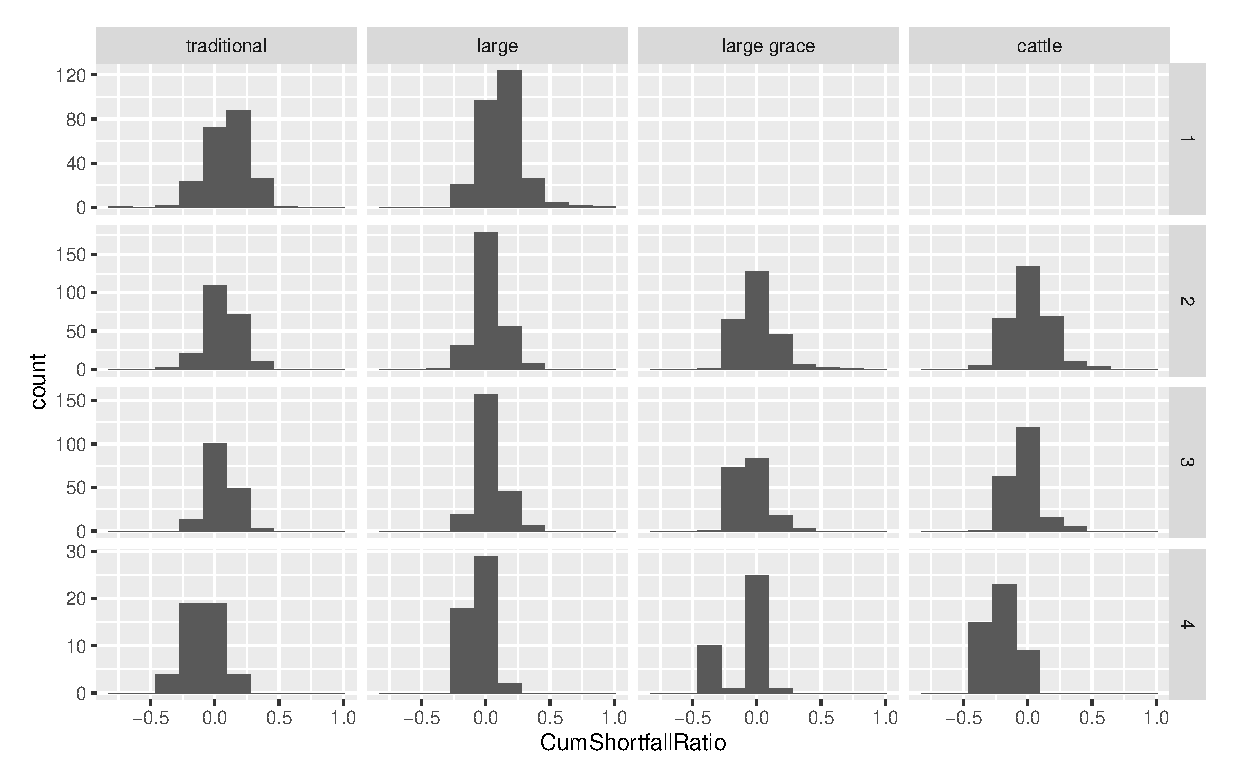
\includegraphics[width=\maxwidth]{PermutationTests5/figureread_shortfall_data-1} 

}

\end{Schunk}
\begin{Schunk}
\begin{Sinput}
RepayPermTestByPoor <- qread(paste0(pathsaveEstimationMemo, "RepayPermTestByPoor.qs"))
X2m <- X2[TeeInLY == 6, .(mean = round(mean(CumShortfallRatio, na.rm = T), 3)), by = .(LoanYear, poor)] 
X2mW <- reshape(X2m, direction  = "wide", idvar = "LoanYear", timevar = "poor")
X2mW[, pvalue := unlist(lapply(RepayPermTestByPoor, 
  function(x) paste0(formatC(coin::midpvalue(x)[1]*100, format = "f", digits = 2), "\\%")))]
numcol <- c("mean.UltraPoor", "mean.ModeratelyPoor")
X2mW[, (numcol) := lapply(.SD, formatC, format = "f", digits = 3), .SDcol = numcol]
X2mW[1:3, mean.UltraPoor := paste0("\\phantom{-}", mean.UltraPoor)]
X2mW[1:3, mean.ModeratelyPoor := paste0("\\phantom{-}", mean.ModeratelyPoor)]
x2mw <- as.matrix(X2mW)
colnames(x2mw) <- c("Loan year", "Ultra poor", "Moderately poor", "") 
x2tab <- latextab(x2mw, 
  hleft = "\\scriptsize\\hfil$", 
  hcenter = c(1, rep(2.25, ncol(x2mw)-1)), 
  hright = "$", 
  headercolor = "gray80", adjustlineskip = "-.2ex", delimiterline= NULL,
  alternatecolor = "gray90",
  addseparatingcols = 2, 
  separatingcolwidth = .1,
  separatingcoltitle = c("Mean cumulative shortfall ratio", "$p$ value"),
  addsubcoltitlehere = T
  )
write.tablev(x2tab,  
  paste0(pathsavePerm, "UltraPoorVsModeratelyPoorRepaymentPermTestResults.tex")
, colnamestrue = F)
\end{Sinput}
\end{Schunk}


\begin{Schunk}
\begin{Sinput}
asv <- readRDS(paste0(pathsaveHere, "DestatData.rds"))
jds <- fread(paste0(pathreceived, "DataForJDS.prn"))
asv[, poor := "Moderately poor"]
asv[hhid %in% jds[grepl("up", pov), hhid], poor := "Ultra poor"]
asv[, poor := factor(poor)]
# asv already dropped anomalous disbursements under trad (776)
asv1 <- asv[!grepl("tw|dou", TradGroup), ]
# drop 2 loan receivers and group rejecters (706)
asv3 <- asv[!grepl("gr", BStatus) & !grepl("tw|dou", TradGroup), ]
X = copy(asv1)
# 
library(coin)
X2[, tradnontrad := "Traditional"]
X2[!grepl("rad", Arm), tradnontrad := "NonTraditional"]
X2[, tradnontrad := factor(tradnontrad, levels = c("Traditional", "NonTraditional"))]

RepayPermTestByArm <- vector(mode = "list", 3)
RepayPermTestByArm <- list(Traditional = RepayPermTestByArm, Cattle = RepayPermTestByArm)

VarsUP <- c("NetValue", "NumCows", "IRejected", "HHsize")
VarsPermTestByPoor <- vector(mode = "list", length(VarsUP))
for (i in 1:length(VarsUP)) 
  VarsPermTestByPoor[[i]] <-  independence_test(
      eval(parse(text=paste0(VarsUP[i], " ~ poor"))), 
      data = X, distribution = approximate(nresample=PermRepTimes)
    )
qsave(VarsPermTestByPoor, 
  paste0(pathsaveEstimationMemo, "VarsPermTestByPoor.qs"))
\end{Sinput}
\end{Schunk}
\begin{Schunk}
\begin{Sinput}
VarsPermTestByPoor <- qread(paste0(pathsaveEstimationMemo, "VarsPermTestByPoor.qs"))

Xm <- X[, .(lapply(.SD,  function(x) round(mean(x, na.rm = T), 3))), 
  .SDcols = VarsUP, by = poor] 
Xo <- X[, .(lapply(.SD,  function(x) round(mean(x, na.rm = T), 3))), 
  .SDcols = VarsUP] 
setnames(Xm, "V1", "val")
setnames(Xo, "V1", "valo")
Xm[, val := as.numeric(val)]
Xm[, vars := rep(VarsUP, 2)]
XmW <- reshape(Xm, direction  = "wide", idvar = "poor", 
  timevar = "vars", v.names = "val")
x2 <- t(XmW)
x2 <- cbind(x2, c("overall", unlist(Xo)))
x2[grepl("NetV", rownames(x2)), ] <- 
  formatC(as.numeric(x2[grepl("NetV", rownames(x2)), ]), format = "f", digits = 0)
x2 <- data.table(variables = rownames(x2), x2)
setnames(x2, c("Variables", "Ultra poor", "Moderately poor", "Overall"))
x2 <- x2[-1, ]
x2[, Variables := gsub("val.", "", Variables)]
x2[, pvalue := unlist(lapply(VarsPermTestByPoor, 
  function(x) paste0(formatC(coin::midpvalue(x)[1]*100, format = "f", digits = 2), "\\%")))]
rn <- x2[, Variables]
source(paste0(pathprogram, "SubstTableANCOVA.R"))
for (i in 1:nrow(subst.tableA)) 
  rn <- gsub(subst.tableA[i, 1], subst.tableA[i, 2], rn)
rn <- paste0("\\makebox[3cm]{\\hfill ", rn, "}")
x2[, Variables := rn]
x2 <- as.matrix(x2)
colnames(x2)[grep("pv", colnames(x2))] <- " " 
x2tab <- latextab(x2, 
  hleft = c("\\hfill\\scriptsize ", rep("\\scriptsize\\hfil$", ncol(x2)-1)), 
  hcenter = c(3, rep(1.75, ncol(x2)-1)), 
  hright = c("", rep("$", ncol(x2)-1)), 
  headercolor = "gray80", adjustlineskip = "-.2ex", delimiterline= NULL,
  alternatecolor = "gray90",
  addseparatingcols = 3, 
  separatingcolwidth = .1,
  separatingcoltitle = c("Mean", "$p$ value"),
  addsubcoltitlehere = T
  )
write.tablev(x2tab,  
  paste0(pathsavePerm, "UltraPoorVsModeratelyPoorBaselineVarsPermTestResults.tex")
, colnamestrue = F)
\end{Sinput}
\end{Schunk}




% This is a child file of PermutationTests5.rnw
\begin{Schunk}
\begin{Sinput}
ar <- readRDS(paste0(pathsaveHere, DataFileNames[3], "Trimmed.rds"))
if (!UseTrimmedSample) ar <- ar[!grepl("tw|dou", TradGroup), ]
if (Only800) ar <- ar[o800 == 1L, ]
# "ar" is roster
# below is what was processed in AttritionTestsContents2.rnw
ar[, Attrited := 1L]
ar[hhid %in% hhid[Time == 4], Attrited := 0L]
ar[, c("Rejected", "GRejected", "IRejected") := 0L]
ar[grepl("^[ig].*rej", BStatus), Rejected := 1L]
ar[grepl("^i.*rej", BStatus), IRejected := 1L]
ar[grepl("^g.*rej", BStatus), GRejected := 1L]
ar[, En := 1:.N, by = .(hhid, Time)]
ar[, Tee := .N, by = .(hhid, mid, Time)]
ar <- ar[En == 1 & Time == 1, ]
\end{Sinput}
\end{Schunk}
Among 776 observations, there are 40 whose villages are washed away and 70 who by group rejected the assigned arms (traditional, large, large grace with 40, 20, 10 individuals, respectively). There are 31, 9, 13, 37 individuals who individually rejected traditional, large, large grace, cattle, respectively. %Among attrited HHs, when were they lost?
\begin{Schunk}
\begin{Sinput}
table(ar[Attrited == 1L, Tee])
\end{Sinput}
\end{Schunk}
%Reasons for attrition and relation to flood damage.
\begin{Schunk}
\begin{Sinput}
table0(ar[Attrited == 1L, .(FloodInRd1, BStatus)])
table0(ar[Attrited == 1L, .(Arm, BStatus)])
\end{Sinput}
\end{Schunk}
% TabLabelStrings is from AttritionPermutationTableHeaders.R in RejectionTestsMainText4.rnw 
% I will modify the table headers for survival/surviving members to "non-attriting borrowers"
%   "survival$", "surviving.*race$", "surv.*other"
\begin{Schunk}
\begin{Sinput}
TabLabelStrings <- 
c(
  "Per.* of rejection$", "of rej.*ng traditional arm$", "of rej.*ng non-traditional arm$", 
  "of rej.*l vs", "p rejection$", "p rej.* traditional arm$", 
  "p rej.*g non-traditional arm$", "p rejecters.*vs", "l rejection$", 
  "l rej.*g tra",  "l rej.*g non-", "l rej.*vs", 
  "bo.*non-ca", 
  "of attrition$", "of attri.* traditional arm$", 
  "of attri.* non-traditional arm$", "of attri.* of",
  "active status$", "active.*race$", "active.*other"
  )
\end{Sinput}
\end{Schunk}
Use \textsf{coin} package's \textsf{independence\_test}: Approximate permutation tests by randomly resampling 100000 times.

% below form permutation tables for all groups examined in AttritionTestContents2.rnw

\begin{Schunk}
\begin{Sinput}
tb1 <- "\\hfil\\begin{minipage}[t]{14cm}\\hfil\\textsc{\\normalsize Table \\refstepcounter{table}\\thetable: "
tb2 <- "}\\\\\\setlength{\\tabcolsep}{.5pt}\\setlength{\\baselineskip}{8pt}\\renewcommand{\\arraystretch}{.50}\\hfil\\begin{tikzpicture}\\node (tbl) {\\input{"
tb3 <- "}};\\end{tikzpicture}\\\\\\begin{tabular}{>{\\hfill\\scriptsize}p{1cm}<{}>{\\hfill\\scriptsize}p{.25cm}<{}>{\\scriptsize}p{12cm}<{\\hfill}}Source:& \\multicolumn{2}{l}{\\scriptsize Estimated with GUK administrative and survey data.}\\\\ Notes: & 1. & \\textsf{R}'s package \\textsf{coin} is used for baseline mean covariates to conduct approximate permutation tests. Number of repetition is set to "
#tb4 <- ". Step-down method is used to adjust for multiple testing of a multi-factor grouping variable. \\textsf{Attrited} and \\textsf{Nonattrited} columns show means of each group. For \\textsf{Arm}, proportions of non-traditional arm are given. \\\\& 2. & ${}^{***}$, ${}^{**}$, ${}^{*}$ indicate statistical significance at 1\\%, 5\\%, 10\\%, respetively. Standard errors are clustered at group (village) level.  \\\\& 3. & See the footnote of \\textsc{Table \\ref{tab MainTextIRjecters}} for description of variables. \\end{tabular}\\end{minipage}\\\\\\vspace{2ex}"
tb42 <- ". Step-down method is used to adjust for multiple testing of a multi-factor grouping variable. The second and third columns show means of each group. For \\textsf{Arm}, proportions of non-traditional arm between two groups are tested. \\\\& 2. & \\textsf{p-value.lower}, \\textsf{p-value.mid}, \\textsf{p-value.upper} indicate lower-bound, mid point value, and upper-bound of the $p$ values for observed test statistic and the null distribution, expressed in per centage units. \\\\& 3. & "
tb41 <- paste(tb42, "See the footnote of \\textsc{Table \\ref{tab MainTextIRjecters}} for description of variables. \\end{tabular}\\end{minipage}\\\\\\vspace{2ex} ")
tb43 <- ".\\\\& 2. &  See footnotes of \\textsc{Table \\ref{tab1 Permutation test results of rejection}}. \\end{tabular}\\end{minipage}\\\\\\vspace{2ex}"
tb44 <- ".\\\\& 2. &  See footnotes of \\textsc{Table \\ref{tab1 Permutation test results of rejection among traditional arm}}. \\end{tabular}\\end{minipage}\\\\\\vspace{2ex}"
tb45 <- paste(tb42, "Contrasts between \\textsf{cattle} arm and other arms. See the footnote of \\textsc{Table \\ref{tab MainTextIRjecters}} for description of variables. \\end{tabular}\\end{minipage}\\\\\\vspace{2ex} ")
for (k in 1:3) 
  for (i in 1:length(HeaderDescription))
    assign(paste0("Tb", k, i), 
      paste0(
        tb1
        , 
        HeaderDescription[i]
        ,
        paste0("\\label{", get(paste0("TabLabel", k))[i], "}")
        ,
        tb2
        , 
        paste0(pathsavePerm, addtofilename[i], c("", "Full", "DropGroupRejecters")[k],
          "PermutationTestResultso800.tex")
        , 
        tb3
        ,
        PermRepTimes
        ,
        #if (i %in% c(1, 5, 11, 17, 21, 25)) tb42 else tb41
        if (i==17) 
          paste0(tb42, TabVariableDescription, PrefTestsDefinitions1, "\\end{tabular}\\end{minipage}\\\\\\vspace{2ex}") else 
        if (i %in% grep("non-catt", HeaderDescription)) # 30, 32 
          tb45 else 
        if (i %in% c(1, 5, 11, 18, 21, 25)) 
          tb43 else 
          tb44
        )
      )
\end{Sinput}
\end{Schunk}

The variables usded: \textsf{Head literate} is an indicator variable of household head literacy. \textsf{Head age} is age of household head. \textsf{Household size} is total number of household members. \textsf{Flood at baseline} is an indicator variable of flood exposure. \textsf{Household asset amount} and \textsf{Productive asset amount} are amount of non-livestock household and productive assets, respectively, in BDT. \textsf{Livestock value} is BDT value of all livestock holding beyond cattle. \textsf{Number of cattle holding} is number of cattle holding. \textsf{Net asset value} is net asset values in BDT using asset items observed in all 4 rounds. \textsf{Broad net asset value} is net asset values in BDT for all asset items. \textsf{Attrited} indicates attrition rates in the household survey, and \textsf{GRejected} and \textsf{IRejected} show group rejection rates and individual rejection rates to the lending program. \textsf{Non-attriting borrowers} indicates the ratio of non-attriting borrowers to all borrowers. Because attrition and rejection are separate events, a household can reject and attrit, so non-attrited borrowers $\geqslant$ total - (rejected members + attrited members). USD 1 is about BDT 80. \textsf{Risk preference} is the respondent's choice of the acceptable minimum excess monetary value of the risky option over a certainty option. Lower values indicate a greater risk tolerance. \textsf{Time preference 1} is the respondent's choice of the acceptable minimum excess monetary value in 3 months that is no smaller than present monetary benefit, and \textsf{Time preference 2} is the the minimum excess value in 1 year and 3 months that is no smaller than monetary benefits of 1 year from now. Lower values indicate a greater patience. If a respondent's \textsf{Time preference 1} is greater than \textsf{Time preference 2}, the respondent is considered to be present-biased. \textsf{Present bias} is an indicator function that takes the value of 1 if the respondent is considered to be present-biased, 0 otherwise. \textsf{Risk preference} is an index where a larger number is associated with more risk tolerance. \textsf{Time preference 1} is an index where a larger number is associated with greater future discounting in a 3 month time frame, and \textsf{Time preference 2} is in a 1 year and 3 month time frame. 
%\textsf{RiskPrefIndex} is an index where a larger number is associated with more risk tolerance. \textsf{TimePref1Index} is an index where a larger number is associated with greater future discounting in a 3 month time frame, and \textsf{TimePref2Index} is in a 1 year and 3 month time frame. \textsf{RiskPrefVal} is the minimum expected monetary value of the risky option that a respondent chose over a certainty option. Lower values indicate a greater risk tolerance. \textsf{TimePref1val} is the respondent's choice of the minimum expected monetary value of future benefits in a 3 month time frame over the present monetary benefit, and \textsf{TimePref2Val} is in a 1 year and 3 month time frame. Lower values indicate a greater patience. If a respondent's \textsf{TimePref1val} is greater than \textsf{TimePref2val}, the respondent is considered to be present-biased. \textsf{PresentBias} is an indicator function that takes the value of 1 if the respondent is considered to be present-biased, 0 otherwise.


\section{Rejection}


\begin{Sinput}
for (i in 1:13) {
  ii <- grep(TabLabelStrings[i], TabLabel1)
  cat(eval(parse(text=paste0("Tb1", ii))))
}
\end{Sinput}
\hfil\begin{minipage}[t]{14cm}\hfil\textsc{\normalsize Table \refstepcounter{table}\thetable: Permutation test results of rejection\label{tab1 Permutation test results of rejection}}\\\setlength{\tabcolsep}{.5pt}\setlength{\baselineskip}{8pt}\renewcommand{\arraystretch}{.50}\hfil\begin{tikzpicture}\node (tbl) {\input{c:/data/GUK/analysis/save/PermutationTests/RejectedPermutationTestResultso800.tex}};\end{tikzpicture}\\\begin{tabular}{>{\hfill\scriptsize}p{1cm}<{}>{\hfill\scriptsize}p{.25cm}<{}>{\scriptsize}p{12cm}<{\hfill}}Source:& \multicolumn{2}{l}{\scriptsize Estimated with GUK administrative and survey data.}\\ Notes: & 1. & \textsf{R}'s package \textsf{coin} is used for baseline mean covariates to conduct approximate permutation tests. Number of repetition is set to 100000. Step-down method is used to adjust for multiple testing of a multi-factor grouping variable. The second and third columns show means of each group. For \textsf{Arm}, proportions of non-traditional arm between two groups are tested. \\& 2. & \textsf{p-value.lower}, \textsf{p-value.mid}, \textsf{p-value.upper} indicate lower-bound, mid point value, and upper-bound of the $p$ values for observed test statistic and the null distribution, expressed in per centage units. \\& 3. & \textsf{Head literate} is an indicator variable of household head literacy. \textsf{Head age} is age of household head. \textsf{Household size} is total number of household members. \textsf{Flood at baseline} is an indicator variable of flood exposure. \textsf{Household asset amount} and \textsf{Productive asset amount} are amount of non-livestock household and productive assets, respectively, in BDT. \textsf{Livestock value} is BDT value of all livestock holding beyond cattle. \textsf{Number of cattle holding} is number of cattle holding. \textsf{Net asset value} is net asset values in BDT using asset items observed in all 4 rounds. \textsf{Broad net asset value} is net asset values in BDT for all asset items. \textsf{Attrited} indicates attrition rates in the household survey, and \textsf{GRejected} and \textsf{IRejected} show group rejection rates and individual rejection rates to the lending program. \textsf{Non-attriting borrowers} indicates the ratio of non-attriting borrowers to all borrowers. Because attrition and rejection are separate events, a household can reject and attrit, so non-attrited borrowers $\geqslant$ total - (rejected members + attrited members). USD 1 is about BDT 80.\textsf{Risk preference} is the respondent's choice of the acceptable minimum excess monetary value of the risky option over a certainty option. Lower values indicate a greater risk tolerance. \textsf{Time preference 1} is the respondent's choice of the acceptable minimum excess monetary value in 3 months that is no smaller than present monetary benefit, and \textsf{Time preference 2} is the the minimum excess value in 1 year and 3 months that is no smaller than monetary benefits of 1 year from now. Lower values indicate a greater patience. If a respondent's \textsf{Time preference 1} is greater than \textsf{Time preference 2}, the respondent is considered to be present-biased. \textsf{Present bias} is an indicator function that takes the value of 1 if the respondent is considered to be present-biased, 0 otherwise.\end{tabular}\end{minipage}\\\vspace{2ex}\hfil\begin{minipage}[t]{14cm}\hfil\textsc{\normalsize Table \refstepcounter{table}\thetable: Permutation test results of rejection among traditional arm\label{tab1 Permutation test results of rejection among traditional arm}}\\\setlength{\tabcolsep}{.5pt}\setlength{\baselineskip}{8pt}\renewcommand{\arraystretch}{.50}\hfil\begin{tikzpicture}\node (tbl) {\input{c:/data/GUK/analysis/save/PermutationTests/RejectedInTradPermutationTestResultso800.tex}};\end{tikzpicture}\\\begin{tabular}{>{\hfill\scriptsize}p{1cm}<{}>{\hfill\scriptsize}p{.25cm}<{}>{\scriptsize}p{12cm}<{\hfill}}Source:& \multicolumn{2}{l}{\scriptsize Estimated with GUK administrative and survey data.}\\ Notes: & 1. & \textsf{R}'s package \textsf{coin} is used for baseline mean covariates to conduct approximate permutation tests. Number of repetition is set to 100000.\\& 2. &  See footnotes of \textsc{Table \ref{tab1 Permutation test results of rejection}}. \end{tabular}\end{minipage}\\\vspace{2ex}\hfil\begin{minipage}[t]{14cm}\hfil\textsc{\normalsize Table \refstepcounter{table}\thetable: Permutation test results of rejection among non-traditional arm\label{tab1 Permutation test results of rejection among non-traditional arm}}\\\setlength{\tabcolsep}{.5pt}\setlength{\baselineskip}{8pt}\renewcommand{\arraystretch}{.50}\hfil\begin{tikzpicture}\node (tbl) {\input{c:/data/GUK/analysis/save/PermutationTests/RejectedInNonTradPermutationTestResultso800.tex}};\end{tikzpicture}\\\begin{tabular}{>{\hfill\scriptsize}p{1cm}<{}>{\hfill\scriptsize}p{.25cm}<{}>{\scriptsize}p{12cm}<{\hfill}}Source:& \multicolumn{2}{l}{\scriptsize Estimated with GUK administrative and survey data.}\\ Notes: & 1. & \textsf{R}'s package \textsf{coin} is used for baseline mean covariates to conduct approximate permutation tests. Number of repetition is set to 100000.\\& 2. &  See footnotes of \textsc{Table \ref{tab1 Permutation test results of rejection among traditional arm}}. \end{tabular}\end{minipage}\\\vspace{2ex}\hfil\begin{minipage}[t]{14cm}\hfil\textsc{\normalsize Table \refstepcounter{table}\thetable: Permutation test results of rejecters, traditional vs. non-traditional arm\label{tab1 Permutation test results of rejecters, traditional vs. non-traditional arm}}\\\setlength{\tabcolsep}{.5pt}\setlength{\baselineskip}{8pt}\renewcommand{\arraystretch}{.50}\hfil\begin{tikzpicture}\node (tbl) {\input{c:/data/GUK/analysis/save/PermutationTests/TradNonTradRejectedPermutationTestResultso800.tex}};\end{tikzpicture}\\\begin{tabular}{>{\hfill\scriptsize}p{1cm}<{}>{\hfill\scriptsize}p{.25cm}<{}>{\scriptsize}p{12cm}<{\hfill}}Source:& \multicolumn{2}{l}{\scriptsize Estimated with GUK administrative and survey data.}\\ Notes: & 1. & \textsf{R}'s package \textsf{coin} is used for baseline mean covariates to conduct approximate permutation tests. Number of repetition is set to 100000.\\& 2. &  See footnotes of \textsc{Table \ref{tab1 Permutation test results of rejection among traditional arm}}. \end{tabular}\end{minipage}\\\vspace{2ex}\hfil\begin{minipage}[t]{14cm}\hfil\textsc{\normalsize Table \refstepcounter{table}\thetable: Permutation test results of group rejection\label{tab1 Permutation test results of group rejection}}\\\setlength{\tabcolsep}{.5pt}\setlength{\baselineskip}{8pt}\renewcommand{\arraystretch}{.50}\hfil\begin{tikzpicture}\node (tbl) {\input{c:/data/GUK/analysis/save/PermutationTests/GRejectedPermutationTestResultso800.tex}};\end{tikzpicture}\\\begin{tabular}{>{\hfill\scriptsize}p{1cm}<{}>{\hfill\scriptsize}p{.25cm}<{}>{\scriptsize}p{12cm}<{\hfill}}Source:& \multicolumn{2}{l}{\scriptsize Estimated with GUK administrative and survey data.}\\ Notes: & 1. & \textsf{R}'s package \textsf{coin} is used for baseline mean covariates to conduct approximate permutation tests. Number of repetition is set to 100000.\\& 2. &  See footnotes of \textsc{Table \ref{tab1 Permutation test results of rejection}}. \end{tabular}\end{minipage}\\\vspace{2ex}\hfil\begin{minipage}[t]{14cm}\hfil\textsc{\normalsize Table \refstepcounter{table}\thetable: Permutation test results of group rejection among traditional arm\label{tab1 Permutation test results of group rejection among traditional arm}}\\\setlength{\tabcolsep}{.5pt}\setlength{\baselineskip}{8pt}\renewcommand{\arraystretch}{.50}\hfil\begin{tikzpicture}\node (tbl) {\input{c:/data/GUK/analysis/save/PermutationTests/GRejectedInTradPermutationTestResultso800.tex}};\end{tikzpicture}\\\begin{tabular}{>{\hfill\scriptsize}p{1cm}<{}>{\hfill\scriptsize}p{.25cm}<{}>{\scriptsize}p{12cm}<{\hfill}}Source:& \multicolumn{2}{l}{\scriptsize Estimated with GUK administrative and survey data.}\\ Notes: & 1. & \textsf{R}'s package \textsf{coin} is used for baseline mean covariates to conduct approximate permutation tests. Number of repetition is set to 100000.\\& 2. &  See footnotes of \textsc{Table \ref{tab1 Permutation test results of rejection among traditional arm}}. \end{tabular}\end{minipage}\\\vspace{2ex}\hfil\begin{minipage}[t]{14cm}\hfil\textsc{\normalsize Table \refstepcounter{table}\thetable: Permutation test results of group rejection among non-traditional arm\label{tab1 Permutation test results of group rejection among non-traditional arm}}\\\setlength{\tabcolsep}{.5pt}\setlength{\baselineskip}{8pt}\renewcommand{\arraystretch}{.50}\hfil\begin{tikzpicture}\node (tbl) {\input{c:/data/GUK/analysis/save/PermutationTests/GRejectedInNonTradPermutationTestResultso800.tex}};\end{tikzpicture}\\\begin{tabular}{>{\hfill\scriptsize}p{1cm}<{}>{\hfill\scriptsize}p{.25cm}<{}>{\scriptsize}p{12cm}<{\hfill}}Source:& \multicolumn{2}{l}{\scriptsize Estimated with GUK administrative and survey data.}\\ Notes: & 1. & \textsf{R}'s package \textsf{coin} is used for baseline mean covariates to conduct approximate permutation tests. Number of repetition is set to 100000.\\& 2. &  See footnotes of \textsc{Table \ref{tab1 Permutation test results of rejection among traditional arm}}. \end{tabular}\end{minipage}\\\vspace{2ex}\hfil\begin{minipage}[t]{14cm}\hfil\textsc{\normalsize Table \refstepcounter{table}\thetable: Permutation test results of group rejecters, traditional vs. non-traditional arm\label{tab1 Permutation test results of group rejecters, traditional vs. non-traditional arm}}\\\setlength{\tabcolsep}{.5pt}\setlength{\baselineskip}{8pt}\renewcommand{\arraystretch}{.50}\hfil\begin{tikzpicture}\node (tbl) {\input{c:/data/GUK/analysis/save/PermutationTests/TradNonTradGRejectedPermutationTestResultso800.tex}};\end{tikzpicture}\\\begin{tabular}{>{\hfill\scriptsize}p{1cm}<{}>{\hfill\scriptsize}p{.25cm}<{}>{\scriptsize}p{12cm}<{\hfill}}Source:& \multicolumn{2}{l}{\scriptsize Estimated with GUK administrative and survey data.}\\ Notes: & 1. & \textsf{R}'s package \textsf{coin} is used for baseline mean covariates to conduct approximate permutation tests. Number of repetition is set to 100000.\\& 2. &  See footnotes of \textsc{Table \ref{tab1 Permutation test results of rejection among traditional arm}}. \end{tabular}\end{minipage}\\\vspace{2ex}\hfil\begin{minipage}[t]{14cm}\hfil\textsc{\normalsize Table \refstepcounter{table}\thetable: Permutation test results of individual rejection\label{tab1 Permutation test results of individual rejection}}\\\setlength{\tabcolsep}{.5pt}\setlength{\baselineskip}{8pt}\renewcommand{\arraystretch}{.50}\hfil\begin{tikzpicture}\node (tbl) {\input{c:/data/GUK/analysis/save/PermutationTests/IRejectedPermutationTestResultso800.tex}};\end{tikzpicture}\\\begin{tabular}{>{\hfill\scriptsize}p{1cm}<{}>{\hfill\scriptsize}p{.25cm}<{}>{\scriptsize}p{12cm}<{\hfill}}Source:& \multicolumn{2}{l}{\scriptsize Estimated with GUK administrative and survey data.}\\ Notes: & 1. & \textsf{R}'s package \textsf{coin} is used for baseline mean covariates to conduct approximate permutation tests. Number of repetition is set to 100000.\\& 2. &  See footnotes of \textsc{Table \ref{tab1 Permutation test results of rejection}}. \end{tabular}\end{minipage}\\\vspace{2ex}\hfil\begin{minipage}[t]{14cm}\hfil\textsc{\normalsize Table \refstepcounter{table}\thetable: Permutation test results of individual rejection among traditional arm\label{tab1 Permutation test results of individual rejection among traditional arm}}\\\setlength{\tabcolsep}{.5pt}\setlength{\baselineskip}{8pt}\renewcommand{\arraystretch}{.50}\hfil\begin{tikzpicture}\node (tbl) {\input{c:/data/GUK/analysis/save/PermutationTests/IRejectedInTradPermutationTestResultso800.tex}};\end{tikzpicture}\\\begin{tabular}{>{\hfill\scriptsize}p{1cm}<{}>{\hfill\scriptsize}p{.25cm}<{}>{\scriptsize}p{12cm}<{\hfill}}Source:& \multicolumn{2}{l}{\scriptsize Estimated with GUK administrative and survey data.}\\ Notes: & 1. & \textsf{R}'s package \textsf{coin} is used for baseline mean covariates to conduct approximate permutation tests. Number of repetition is set to 100000.\\& 2. &  See footnotes of \textsc{Table \ref{tab1 Permutation test results of rejection among traditional arm}}. \end{tabular}\end{minipage}\\\vspace{2ex}\hfil\begin{minipage}[t]{14cm}\hfil\textsc{\normalsize Table \refstepcounter{table}\thetable: Permutation test results of individual rejection among non-traditional arm\label{tab1 Permutation test results of individual rejection among non-traditional arm}}\\\setlength{\tabcolsep}{.5pt}\setlength{\baselineskip}{8pt}\renewcommand{\arraystretch}{.50}\hfil\begin{tikzpicture}\node (tbl) {\input{c:/data/GUK/analysis/save/PermutationTests/IRejectedInNonTradPermutationTestResultso800.tex}};\end{tikzpicture}\\\begin{tabular}{>{\hfill\scriptsize}p{1cm}<{}>{\hfill\scriptsize}p{.25cm}<{}>{\scriptsize}p{12cm}<{\hfill}}Source:& \multicolumn{2}{l}{\scriptsize Estimated with GUK administrative and survey data.}\\ Notes: & 1. & \textsf{R}'s package \textsf{coin} is used for baseline mean covariates to conduct approximate permutation tests. Number of repetition is set to 100000.\\& 2. &  See footnotes of \textsc{Table \ref{tab1 Permutation test results of rejection among traditional arm}}. \end{tabular}\end{minipage}\\\vspace{2ex}\hfil\begin{minipage}[t]{14cm}\hfil\textsc{\normalsize Table \refstepcounter{table}\thetable: Permutation test results of individual rejecters, traditional vs. non-traditional arm\label{tab1 Permutation test results of individual rejecters, traditional vs. non-traditional arm}}\\\setlength{\tabcolsep}{.5pt}\setlength{\baselineskip}{8pt}\renewcommand{\arraystretch}{.50}\hfil\begin{tikzpicture}\node (tbl) {\input{c:/data/GUK/analysis/save/PermutationTests/TradNonTradIRejectedPermutationTestResultso800.tex}};\end{tikzpicture}\\\begin{tabular}{>{\hfill\scriptsize}p{1cm}<{}>{\hfill\scriptsize}p{.25cm}<{}>{\scriptsize}p{12cm}<{\hfill}}Source:& \multicolumn{2}{l}{\scriptsize Estimated with GUK administrative and survey data.}\\ Notes: & 1. & \textsf{R}'s package \textsf{coin} is used for baseline mean covariates to conduct approximate permutation tests. Number of repetition is set to 100000.\\& 2. &  See footnotes of \textsc{Table \ref{tab1 Permutation test results of rejection among traditional arm}}. \end{tabular}\end{minipage}\\\vspace{2ex}\hfil\begin{minipage}[t]{14cm}\hfil\textsc{\normalsize Table \refstepcounter{table}\thetable: Permutation test results of borrowers, cattle vs. non-cattle arms\label{tab1 Permutation test results of borrowers, cattle vs. non-cattle arms}}\\\setlength{\tabcolsep}{.5pt}\setlength{\baselineskip}{8pt}\renewcommand{\arraystretch}{.50}\hfil\begin{tikzpicture}\node (tbl) {\input{c:/data/GUK/analysis/save/PermutationTests/AcceptedCowNonCowPermutationTestResultso800.tex}};\end{tikzpicture}\\\begin{tabular}{>{\hfill\scriptsize}p{1cm}<{}>{\hfill\scriptsize}p{.25cm}<{}>{\scriptsize}p{12cm}<{\hfill}}Source:& \multicolumn{2}{l}{\scriptsize Estimated with GUK administrative and survey data.}\\ Notes: & 1. & \textsf{R}'s package \textsf{coin} is used for baseline mean covariates to conduct approximate permutation tests. Number of repetition is set to 100000. Step-down method is used to adjust for multiple testing of a multi-factor grouping variable. The second and third columns show means of each group. For \textsf{Arm}, proportions of non-traditional arm between two groups are tested. \\& 2. & \textsf{p-value.lower}, \textsf{p-value.mid}, \textsf{p-value.upper} indicate lower-bound, mid point value, and upper-bound of the $p$ values for observed test statistic and the null distribution, expressed in per centage units. \\& 3. &  Contrasts between \textsf{cattle} arm and other arms. See the footnote of \textsc{Table \ref{tab MainTextIRjecters}} for description of variables. \end{tabular}\end{minipage}\\\vspace{2ex} 

%	\noindent\textsc{\normalsize Table \ref{grep(TabLabelStrings[1], TabLabel1)}} to \textsc{\normalsize Table \ref{grep(TabLabelStrings[13], TabLabel1)}}: Trimmed sample.\\

	\textsc{\normalsize Table \ref{tab1 Permutation test results of rejection}} shows test results of independence between loan receivers and nonreceivers (group, individual rejecters) on the analysis sample of 776 members. It shows that lower head literacy, smaller household size, being affected by flood at the baseline, smaller cattle/livestock holding, and smaller net assets are correlated with opting out the offered type of lending. Smaller net assets based on broader items also show a tendency to reject a participation offer. \textsf{Risk preference} indicates that the minimum expected payoff to choose a risky option is greater, albeit to a small degree, for the rejecters. Time preference variables show statistically indistinguishable differences. Ratio of \textsf{PresentBias} is high but there is no statistically large difference between the two groups.
	\textsc{\normalsize Table \ref{tab1 Permutation test results of rejection among traditional arm}} indicates that contrasts of smaller net asset holding and cattle/livestock holding are more pronounced among \textsf{traditional} rejecters than in the case of all rejecters of \textsc{\normalsize Table \ref{tab1 Permutation test results of rejection}}. It also shows that flood exposure among the rejecters is less frequent than in \textsc{\normalsize Table \ref{tab1 Permutation test results of rejection}}. 
	\textsc{\normalsize Table \ref{tab1 Permutation test results of rejection among non-traditional arm}} indicates that lower head literacy, smaller household size, higher flood exposure, are more pronounced among non-\textsf{traditional} rejecters than in the case of all rejecters of \textsc{\normalsize Table \ref{tab1 Permutation test results of rejection}}. \textsf{Risk preference} shows greater risk torelance among non-rejeceters than rejecters of the non-\textsf{traditional} arms. It also shows that asset and livestock holding is not statistically different between rejecters and non-rejecters. The only difference between rejecters of \textsf{traditional} and non-\textsf{traditiona} arms we observe in \textsc{\normalsize Table \ref{tab1 Permutation test results of rejecters, traditional vs. non-traditional arm}}is lower flood exposure of the former. Due possibly to a small sample size, smaller asset and livestock holding of the \textsf{traditional} arm rejecters is merely suggestive. 
	
	Group rejecters and non-group rejecters are compared in \textsc{\normalsize Table \ref{tab1 Permutation test results of group rejection}}. Marked differences are found in arm (\textsf{traditional} vs. non-\textsf{traditional}) and net asset values and head literacy are noted. We see more \textsf{PresentBias} in the group-rejecters. This is difficult to understand but is consistent with the situation that the rejection decision was made because procrastination of some members can lead to loan defaults which causes a problem to the group as a whole. As we will see later, the comparison of individual rejecters and non-rejecters do not show such a difference in \textsf{PresentBias}. This is also consistent with such a `group wariness' interpretation. \textsc{\normalsize Table \ref{tab1 Permutation test results of group rejection among traditional arm}} compares group rejecters in \textsf{traditional} arm and finds smaller flood exposure and lower livestock and net asset holding are associated with group rejection. Group rejecters in non-\textsf{traditional} arm are examined in \textsc{\normalsize Table \ref{tab1 Permutation test results of group rejection among non-traditional arm}} and younger head age, flood at baseline, and smaller household asset holding are correlated with rejection. Comparing group rejecters between \textsf{traditional} and non-\textsf{traditional} arms in \textsc{\normalsize Table \ref{tab1 Permutation test results of group rejecters, traditional vs. non-traditional arm}}, younger head age, higher flood exposure, larger net asset values and livestock holding are noted among the non-\textsf{traditional} group rejecters. These hint that for non-\textsf{traditional} arm group rejecters, it is the smaller household size and the baseline flood that may have constrained them from participation, and for \textsf{traditional} group rejecters, it is the low asset levels.

	Acknowledging the reasons for rejection can be different, we tested the independence of each characteristics for individual rejecters (vs. participants) in \textsc{\normalsize Table \ref{tab1 Permutation test results of individual rejection}}. Smaller \textsf{HHsize}, being affected with \textsf{FloodInRd1}, and smaller \textsf{LivestockValue}, \textsf{NumCows}, and \textsf{NetValue} are associated with individual rejecters. Individual decisions not to participate may be more straightforward: Smaller household size may indicate difficulty in securing the cattle production labour in a household, being hit with a flood may have resulted in lower livestock levels that would prompt them to reconsider partaking in another livestock project. Individual rejecters exhibit smaller risk tolerance, which was not observed among the group rejecters. This also fortifies the disadvantages of having less favourable conditions in terms of household size, asset positions, and shocks.

	\textsc{\normalsize Table \ref{tab1 Permutation test results of individual rejection among traditional arm}} and \textsc{\normalsize Table \ref{tab1 Permutation test results of individual rejection among non-traditional arm}} compare individual rejecters and nonrejecters in \textsf{traditional} arm and non-\textsf{traditional} arms, respectively. For \textsf{traditional} rejecters, livestock and other asset values are not correlated with rejection, but the values are similar to non-\textsf{traditional} and higher $p$ values may be due to smaller sample size. For non-\textsf{traditional} arm rejecters, household size and flood exposure are correlated. Comparison of individual rejecters between \textsf{traditional} and non-\textsf{traditional} arms show no detectable difference (\textsc{\normalsize Table \ref{tab1 Permutation test results of individual rejecters, traditional vs. non-traditional arm}}). This suggests that indvidual rejecters in all arms were constrained with small household size and small asset holding. In \textsc{\normalsize Table \ref{tab1 Permutation test results of borrowers, cattle vs. non-cattle arms}}, we compare if the \textsf{cattle} arm participants (borrowers) differ from participants in other arms at the baseline. It is worth noting that partcipants of \textsf{cattle} arm differ from other arms in having less cattle rearing experience as observed in smaller initial cattle holding ($p$ value = .156) and in having lower net asset values ($p$ value = .058), weakly hinting that the \textsf{cattle} arm's managerial support programs may have encouraged participation of inexperienced or lower asset holders. \label{RejectionLastPage}

	%	A closer look at the nonparticipation correlates among \textsf{traditional} arm mebers in \textsc{\normalsize Table \ref{tab reject trad perm}} and non-\textsf{traditional} arm members in \textsc{\normalsize Table \ref{tab reject nontrad perm}} reveal possible differences in the causes. Rejection among \textsf{traditional} members tend to be associated with lower livestock holding but not with higher flood exposure nor smaller household size, while rejecters among non-\textsf{traditional} members are more likely to have suffered from flood in baseline and have smaller household size. Since the offered arms were randomised, rejecters of \textsf{traditional} arm, who were not more exposed to flood and have similar household size at the mean, may have accepted the offer had they been offered non- \textsf{traditional} lending. Henceforth, we conjecture that flood exposure and household size are the potential impediments in larger size loans. This implies that there may not be minimum livestock and asset holding levels to partake the larger loans, and a poverty trap at this level may be overcome.

\section{Attrition}

\begin{Schunk}
\begin{Sinput}
HeaderDescription[11:16] <- c(
   "Permutation test results of attrition among borrowers", 
     "Permutation test results of attrition among traditional arm borrowers",
     "Permutation test results of attrition among non-traditional arm borrowers",
     "Permutation test results of non-attriting members of traditional and non-traditional arm borrowers",
     "Permutation test results of non-attriting members of cattle and all other arm borrowers",
     "Permutation test results of non-attriting members of cattle and large grace arm borrowers",
    )
TabLabel1 <- paste("tab1", HeaderDescription)
\end{Sinput}
\end{Schunk}

\begin{Schunk}
\begin{Sinput}
TabLabelStrings[19:20] <- c("active.*race arms$", "acti.*other arms$")
\end{Sinput}
\end{Schunk}
\begin{Sinput}
for (i in 14:length(TabLabelStrings)) {
  ii <- grep(TabLabelStrings[i], TabLabel1)
  if (grepl("active status", TabLabelStrings[i])){
   tblatt <- eval(parse(text=paste0("Tb1", ii)))
   cat(gsub("active\\\\", "attrited or rejected (NonActive) and other (Active) borrowers\\\\", 
     tblatt)) 
   rm(tblatt)
  } else
  if (grepl("active ra|acti.*o", TabLabelStrings[i])) {
   tblatt <- eval(parse(text=paste0("Tb1", ii)))
   cat(#gsub("active members", "non-active borrowers", 
     tblatt
     #)
     ) 
    rm(tblatt)
  } else
   cat(eval(parse(text=paste0("Tb1", ii))))
}
\end{Sinput}
\hfil\begin{minipage}[t]{14cm}\hfil\textsc{\normalsize Table \refstepcounter{table}\thetable: Permutation test results of attrition\label{tab1 Permutation test results of attrition}}\\\setlength{\tabcolsep}{.5pt}\setlength{\baselineskip}{8pt}\renewcommand{\arraystretch}{.50}\hfil\begin{tikzpicture}\node (tbl) {\input{c:/data/GUK/analysis/save/PermutationTests/AttritedPermutationTestResultso800.tex}};\end{tikzpicture}\\\begin{tabular}{>{\hfill\scriptsize}p{1cm}<{}>{\hfill\scriptsize}p{.25cm}<{}>{\scriptsize}p{12cm}<{\hfill}}Source:& \multicolumn{2}{l}{\scriptsize Estimated with GUK administrative and survey data.}\\ Notes: & 1. & \textsf{R}'s package \textsf{coin} is used for baseline mean covariates to conduct approximate permutation tests. Number of repetition is set to 100000.\\& 2. &  See footnotes of \textsc{Table \ref{tab1 Permutation test results of rejection}}. \end{tabular}\end{minipage}\\\vspace{2ex}\hfil\begin{minipage}[t]{14cm}\hfil\textsc{\normalsize Table \refstepcounter{table}\thetable: Permutation test results of attrition among traditional arm\label{tab1 Permutation test results of attrition among traditional arm}}\\\setlength{\tabcolsep}{.5pt}\setlength{\baselineskip}{8pt}\renewcommand{\arraystretch}{.50}\hfil\begin{tikzpicture}\node (tbl) {\input{c:/data/GUK/analysis/save/PermutationTests/AttritedInTradPermutationTestResultso800.tex}};\end{tikzpicture}\\\begin{tabular}{>{\hfill\scriptsize}p{1cm}<{}>{\hfill\scriptsize}p{.25cm}<{}>{\scriptsize}p{12cm}<{\hfill}}Source:& \multicolumn{2}{l}{\scriptsize Estimated with GUK administrative and survey data.}\\ Notes: & 1. & \textsf{R}'s package \textsf{coin} is used for baseline mean covariates to conduct approximate permutation tests. Number of repetition is set to 100000.\\& 2. &  See footnotes of \textsc{Table \ref{tab1 Permutation test results of rejection among traditional arm}}. \end{tabular}\end{minipage}\\\vspace{2ex}\hfil\begin{minipage}[t]{14cm}\hfil\textsc{\normalsize Table \refstepcounter{table}\thetable: Permutation test results of attrition among non-traditional arm\label{tab1 Permutation test results of attrition among non-traditional arm}}\\\setlength{\tabcolsep}{.5pt}\setlength{\baselineskip}{8pt}\renewcommand{\arraystretch}{.50}\hfil\begin{tikzpicture}\node (tbl) {\input{c:/data/GUK/analysis/save/PermutationTests/AttritedInNonTradPermutationTestResultso800.tex}};\end{tikzpicture}\\\begin{tabular}{>{\hfill\scriptsize}p{1cm}<{}>{\hfill\scriptsize}p{.25cm}<{}>{\scriptsize}p{12cm}<{\hfill}}Source:& \multicolumn{2}{l}{\scriptsize Estimated with GUK administrative and survey data.}\\ Notes: & 1. & \textsf{R}'s package \textsf{coin} is used for baseline mean covariates to conduct approximate permutation tests. Number of repetition is set to 100000.\\& 2. &  See footnotes of \textsc{Table \ref{tab1 Permutation test results of rejection among traditional arm}}. \end{tabular}\end{minipage}\\\vspace{2ex}\hfil\begin{minipage}[t]{14cm}\hfil\textsc{\normalsize Table \refstepcounter{table}\thetable: Permutation test results of attriters of traditional and non-traditional arms\label{tab1 Permutation test results of attriters of traditional and non-traditional arms}}\\\setlength{\tabcolsep}{.5pt}\setlength{\baselineskip}{8pt}\renewcommand{\arraystretch}{.50}\hfil\begin{tikzpicture}\node (tbl) {\input{c:/data/GUK/analysis/save/PermutationTests/TradNonTradAttritedPermutationTestResultso800.tex}};\end{tikzpicture}\\\begin{tabular}{>{\hfill\scriptsize}p{1cm}<{}>{\hfill\scriptsize}p{.25cm}<{}>{\scriptsize}p{12cm}<{\hfill}}Source:& \multicolumn{2}{l}{\scriptsize Estimated with GUK administrative and survey data.}\\ Notes: & 1. & \textsf{R}'s package \textsf{coin} is used for baseline mean covariates to conduct approximate permutation tests. Number of repetition is set to 100000.\\& 2. &  See footnotes of \textsc{Table \ref{tab1 Permutation test results of rejection among traditional arm}}. \end{tabular}\end{minipage}\\\vspace{2ex}\hfil\begin{minipage}[t]{14cm}\hfil\textsc{\normalsize Table \refstepcounter{table}\thetable: Permutation test results of active status\label{tab1 Permutation test results of active status}}\\\setlength{\tabcolsep}{.5pt}\setlength{\baselineskip}{8pt}\renewcommand{\arraystretch}{.50}\hfil\begin{tikzpicture}\node (tbl) {\input{c:/data/GUK/analysis/save/PermutationTests/ActivePermutationTestResultso800.tex}};\end{tikzpicture}\\\begin{tabular}{>{\hfill\scriptsize}p{1cm}<{}>{\hfill\scriptsize}p{.25cm}<{}>{\scriptsize}p{12cm}<{\hfill}}Source:& \multicolumn{2}{l}{\scriptsize Estimated with GUK administrative and survey data.}\\ Notes: & 1. & \textsf{R}'s package \textsf{coin} is used for baseline mean covariates to conduct approximate permutation tests. Number of repetition is set to 100000.\\& 2. &  See footnotes of \textsc{Table \ref{tab1 Permutation test results of rejection}}. \end{tabular}\end{minipage}\\\vspace{2ex}\hfil\begin{minipage}[t]{14cm}\hfil\textsc{\normalsize Table \refstepcounter{table}\thetable: Permutation test results of active members of cattle and large grace arms\label{tab1 Permutation test results of active members of cattle and large grace arms}}\\\setlength{\tabcolsep}{.5pt}\setlength{\baselineskip}{8pt}\renewcommand{\arraystretch}{.50}\hfil\begin{tikzpicture}\node (tbl) {\input{c:/data/GUK/analysis/save/PermutationTests/ActiveCowLargeGracePermutationTestResultso800.tex}};\end{tikzpicture}\\\begin{tabular}{>{\hfill\scriptsize}p{1cm}<{}>{\hfill\scriptsize}p{.25cm}<{}>{\scriptsize}p{12cm}<{\hfill}}Source:& \multicolumn{2}{l}{\scriptsize Estimated with GUK administrative and survey data.}\\ Notes: & 1. & \textsf{R}'s package \textsf{coin} is used for baseline mean covariates to conduct approximate permutation tests. Number of repetition is set to 100000.\\& 2. &  See footnotes of \textsc{Table \ref{tab1 Permutation test results of rejection among traditional arm}}. \end{tabular}\end{minipage}\\\vspace{2ex}\hfil\begin{minipage}[t]{14cm}\hfil\textsc{\normalsize Table \refstepcounter{table}\thetable: Permutation test results of active members of cattle and all other arms\label{tab1 Permutation test results of active members of cattle and all other arms}}\\\setlength{\tabcolsep}{.5pt}\setlength{\baselineskip}{8pt}\renewcommand{\arraystretch}{.50}\hfil\begin{tikzpicture}\node (tbl) {\input{c:/data/GUK/analysis/save/PermutationTests/ActiveCowNonCowPermutationTestResultso800.tex}};\end{tikzpicture}\\\begin{tabular}{>{\hfill\scriptsize}p{1cm}<{}>{\hfill\scriptsize}p{.25cm}<{}>{\scriptsize}p{12cm}<{\hfill}}Source:& \multicolumn{2}{l}{\scriptsize Estimated with GUK administrative and survey data.}\\ Notes: & 1. & \textsf{R}'s package \textsf{coin} is used for baseline mean covariates to conduct approximate permutation tests. Number of repetition is set to 100000.\\& 2. &  See footnotes of \textsc{Table \ref{tab1 Permutation test results of rejection among traditional arm}}. \end{tabular}\end{minipage}\\\vspace{2ex}
% uptake: 105+171+177+163
% rejected: rjcted <- 71+29+23+37
% attrited: 32+8+29+23
% borrower nonattriting (survivors): 83+164+160+147=83+164+160+147
% borrower attriting: boratt <- (105-83)+(171-164)+(177-160)+(163-147)
% nonborrower nonattriting: 61+28+11+30
% nonborrower attriting: (40+31-36-25)+(20+9-19-9)+(10+13-11)+(37-39)
% rejected or attrited (nonsurvivors): borrower attriting + rejected = boratt + rjcted

	\textsc{\normalsize Table \ref{tab1 Permutation test results of attrition}} shows results from tests of independence between attriters and nonattriters. Attrition is defined as attrition from household surveys, not from the lending program. We see the moderate rate of attrition is not correlated with household level characteristics%, except less risk torelance in \textsf{RiskPrefVal}, 
	at the conventional $p$ value level. Productive asset amounts seem to differ between attriters and nonattriters at $p=.105$, with the former being larger than the latter. This positive attrition selection can cause underestimation of impacts, if the asset values are positively correlated with entrepreneurial capacity. We also see that the attriters are less risk tolerant in terms of minimum expected payoff to choose a risky option in \textsf{RiskPrefVal}. \textsc{\normalsize Table \ref{tab1 Permutation test results of attrition among traditional arm}} shows attrition in the \textsf{traditional} arm. Household heads of attriters are relatively less literate than nonattriters. We observe the \textsf{traditional} arm attriters are less risk tolerant the nonattriters.
	\textsc{\normalsize Table \ref{tab1 Permutation test results of attrition among non-traditional arm}} compares attriters and nonattriters in the non-\textsf{traditional} arm. Unlike \textsf{traditional} arm attriters, non-\textsf{traditional} arm attriters have more literate household heads, have a larger household size, are more exposed to floods, and have larger productive assets. The \textsf{traditional} arm attriters may be less entrepreneurial, if anything, so their attrition may upwardly bias the positive gains of the arm, hence understate the impacts of non-\textsf{traditional} arm. These are explicitly shown in \textsc{\normalsize Table \ref{tab1 Permutation test results of attriters of traditional and non-traditional arms}} where we compare attriters of \textsf{traditional} and non-\textsf{traditional} arms. Overall, attrition may have attenuated the impacts but is not likely to have inflated them.\footnote{So one can employ the Lee bounds for stronger results, but doing so will give us less precision and require more assumptions. We will not use the Lee bounds \textcolor{red}{[we can show them if necessary]}. } We observe the non-\textsf{traditional} arm attriters are also less risk tolerant than the nonattriters.

	For the microfinance institutions (MFIs), attrition of the loan receiving members poses a threat to their business continuation. Financial institutions often use observable characteristics, such as collateralisable assets, and easily surveyed chracteristics, such as job experiences and schooling of borrowers, and are likely to lend if the assets levels are greater and the borrowers have relevant job experiences and more schooling. We first examine if such screening variables have any predictive power in terms of loan rejection or borrower attrition under our lending. \textsc{\normalsize Table \ref{tab1 Permutation test results of active status}} compares potential MFI targets (nonattriting borrowers, noted as \textsf{Active}) vs. non-targets (attriting borrowers or loan rejecters, noted as \textsf{NonActive}) in all arms. It shows potential targets at the baseline have larger values in livestock and greater number of cattle, and are less affected by the flood, which conforms the conventional wisdom of lenders in using these aspects in their loan decisions. We also see that more risk torelant members are likely to be borrowers and do not attrit. Next, we examine if the relationship of having ``less favourable'' values in these characteristics and attrition is mitigated under various loan characteristics. In \textsc{\normalsize Table \ref{tab1 Permutation test results of active members of cattle and large grace arms}}, we restrict our attention to the potential MFI targets, or the nonattriting borrowers, and compare between \textsf{cattle} and \textsf{large grace} arms, whose difference is efffectively the presence of managerial supports that the former provides. \label{PageOfAttrition}%Comparing the nonattriting borrower, characteristics are similar except that the \textsf{traditional} members are more exposed to the flood than the non-\textsf{traditional} members. 
	Comparing against the \textsf{large grace} arm, nonattriting borrowers of the \textsf{cattle} arm are more exposed to the flood ($p=.055$), have less productive assets ($p=.003$), have lower net asset values ($p=.046$), and have fewer livestock ($p=.139$). This shows that the smaller livestock holders or individuals with less experienced in livestock are encouraged to participate and continue to operate in the \textsf{cattle} arm that has a managerial support program, with all other features being equal. This is consistent with our analysis of participation in \textsc{\normalsize Table \ref{tab1 Permutation test results of borrowers, cattle vs. non-cattle arms}} which weakly hints that the \textsf{cattle} arm's managerial support programs may have encouraged participation of inexperienced or lower asset holders. This also underscores our interpretation that the current impact estimates may be downwardly biased, if any, as people who would otherwise attrit or reject in the \textsf{cattle} arm stayed on. This result is confirmed with lower $p$ values due to a larger sample size when we compare the nonattriting borrowers between \textsf{cattle} arm with all other arms in \textsc{\normalsize Table \ref{tab1 Permutation test results of active members of cattle and all other arms}}. At the baseline, \textsf{cattle} arm nonattriting borrowers have smaller baseline livestock holding ($p$ value = .016) and smaller baseline net asset holding ($p$ value = .007) than other arms' nonattriting borrowers. 

%	Moved from main text.
	
%	Group rejecters of \textsf{traditional} and non-\textsf{traditional} arms differ in household characteristics. Lower livestock values, smaller cattle holding, and smaller net asset values are associated with group rejection for \textsf{traditional} arm (\textsc{\normalsize Table \ref{TabLabel1[grep("p rej.* traditional arm$", TabLabel1)]}}), while higher baseline flood exposure rates and younger household heads are associated with group rejection for non-\textsf{traditional} arms (\textsc{\normalsize Table \ref{TabLabel1[grep("p rej.*g non-traditional arm$", TabLabel1)]}}). Given randomisation, we conjecture that it is lack of \textsf{Upfront} liquidity that prevented smaller livestock holders of \textsf{traditional} arm from participating because they cannot purchase cattle due to insufficient net asset values or an insufficient resale value of owned livestock, when members of similar characteristics partcipated in non-\textsf{traditional} arms. %This is a real resource constraint that binds the households. This is different from a psychological constraint that, so long as there is a cost or a payment involved, albeit at a minimal level, there remains a group of households who would not take up the investment \citep{Ashraf2010, CohenDupas2010}. 
%	For non-\textsf{traditional} arm rejecters, it is the past flood that kept members from participating, even they are younger and have similar cattle holding as the non group-rejecters. 

%	Individual rejecters of \textsf{traditional} arm and non-\textsf{traditional} arms share similar characteristics (\textsc{\normalsize Table \ref{TabLabel1[grep("l rej.*vs", TabLabel1)]}}). In fact, they are not very different in all the variables considered. %This is consistent with the conjecture that, had the \textsf{traditional} arm group rejecters been offered any of the non-\textsf{traditional} arms, they, as a group, may have accepted it.  %It shows the latter is more exposed to flood in baseline and has larger livestock values. This implies that, once large enough sum of loan is disbursed, %there is no minimum livestock and asset holding level to partake in the larger loans, and 
	%despite a negative asset shock in flood and a poverty trap at this level may be overcome once household size and negative asset shocks are accounted for.
%	The common factors associated with nonparticipation are a smaller household size and smaller livestock holding (\textsc{\normalsize Table \ref{TabLabel1[grep("l rej.*g tra", TabLabel1)]}} and \textsc{\normalsize Table \ref{TabLabel1[grep("l rej.*g non-", TabLabel1)]}}), although the $p$ values for livestock holding difference between individual rejecters and non individual rejecters are around 7\% (\textsc{\normalsize Table \ref{TabLabel1[grep("l rejection$", TabLabel1)]}}). %In non-\textsf{traditional} arms, the individual rejecters have only marginally different mean values relative to individual nonrejecters (\textsc{\normalsize Table \ref{tab Ireject nontrad perm}}). 



\end{document}
